\documentclass[11pt]{article}

\pdfoptionpdfminorversion=5

% American letter size:
\textwidth6.5in \textheight9in \oddsidemargin 0pt \evensidemargin 0pt
\topmargin -47pt


\usepackage{times}
\usepackage{fullpage}
\usepackage{epic}
\usepackage{subfigure}
\usepackage{wrapfig}
\usepackage{eepic}
\usepackage{epsfig}
\usepackage{color}
\usepackage{amsmath,amsthm,amssymb}
\usepackage{amsfonts}
\usepackage{float}
\usepackage{appendix}
\usepackage{multirow}
\usepackage{booktabs}
\usepackage{url}

\renewcommand\floatpagefraction{1.0}
\renewcommand\topfraction{1.0}
\renewcommand\bottomfraction{0.9}
\renewcommand\bottomfraction{1.0}
\renewcommand\textfraction{0.0}

\newenvironment{enum*}%
 {\begin{enumerate}%
   \setlength{\itemsep}{-5pt}%
   \setlength{\parsep}{-5pt}%
   \setlength{\topsep}{-5pt}}%
 {\end{enumerate}}

\newenvironment{item*}%
 {\begin{itemize}%
   \setlength{\itemsep}{-5pt}%
   \setlength{\parsep}{-5pt}%
   \setlength{\topsep}{-5pt}}%
 {\end{itemize}}

\newcommand{\tup}[1]{%
        \relax\ifmmode
	           \langle #1 \rangle%
        \else
                $\langle$#1$\rangle$%
        \fi
}

\theoremstyle{plain}
\floatstyle{ruled}
\newfloat{algo}{htbp}{algo}
\floatname{algo}{Algorithm}
\usepackage[noend]{algorithmic}
\usepackage{distribalgo}

\usepackage{setspace}
%\doublespacing

\newtheorem{thm}{Theorem}
\newtheorem{lemma}{Lemma}
\newtheorem{claim}{Claim}
\newtheorem{corollary}{Corollary}
\newtheorem{definition}{Definition}
\newtheorem{property}{Property}
\newtheorem{proposition}{Proposition}
\newtheorem{observation}{Observation}
\newtheorem{conjecture}{Conjecture}
\newtheorem{designrule}{Design Principle}
\newtheorem{invariant}{Invariant}
\newtheorem{theorem}{Theorem}

\newcommand{\up}[1]{\ensuremath{^{\textrm{#1}}}}
\newcommand{\down}[1]{\ensuremath{_{\textrm{#1}}}}
\newcommand{\tb}{\makebox[0.6cm]{}}
\newcommand{\negspace}{\vspace{-0.6\baselineskip}}
\newcommand{\snegspace}{\vspace{-0.25\baselineskip}}
\def\hyph{-\penalty0\hskip0pt\relax}

\newenvironment{restate}[1]{\begin{trivlist} \item {\bf #1 (restated)} \em}
  {\end{trivlist}}

\definecolor{Gray}{rgb}{0.1,0.4,0.1}
\definecolor{DarkBlue}{rgb}{0.2,0.2,0.5}
\definecolor{Cyan}{rgb}{0.5,0.2,0.5}
\newcommand{\comment}[1]{{\color{Gray}{$\rhd$ #1}}}
\newcommand{\elcomment}[1]{\hfill{\comment{#1}}}
\newcommand{\funcname}[1]{\textsc{\color{DarkBlue}{#1}}}
\newcommand{\typename}[1]{\textbf{\color{Cyan}{#1}}}

\setlength\topmargin{-0.025in}
\setlength\textheight{8.75in}

%%=======================================================================
%% Latex template for SPAA 2012
%%=======================================================================
%
%% remember to compile with dvips -t letter for US letter style
%
%\documentclass[11pt]{article}
%
%% American letter size:
%\textwidth6.5in \textheight9in \oddsidemargin 0pt \evensidemargin 0pt
%\topmargin -47pt
%
%\usepackage{times}
%
%\newtheorem{theorem}{Theorem}[section]
%\newtheorem{lemma}[theorem]{Lemma}
%\newtheorem{claim}[theorem]{Claim}
%\newtheorem{fact}[theorem]{Fact}
%
%\newcommand{\sq}{\hbox{\rlap{$\sqcap$}$\sqcup$}}
%\newcommand{\qed}{\hspace*{\fill}\sq}
%\newenvironment{proof}{\noindent {\bf Proof.}\ }{\qed\par\vskip 4mm\par}
%\newenvironment{proofof}[1]{\bigskip \noindent {\bf Proof of #1:}\quad }
%{\qed\par\vskip 4mm\par}



\begin{document}

\begin{titlepage}

\title{SALSA: Scalable and Low Synchronization NUMA-aware Algorithm for Producer-Consumer Pools \\
       {\Large (Regular Submission)}}

\author{Elad Gidron \\
   Department of Computer Science,\\Technion, Haifa, Israel\\
   eladgi@cs.technion.ac.il \\
   \and
   Idit Keidar \\
   Department of Electrical Engineering,\\Technion, Haifa, Israel\\
   idish@ee.technion.ac.il \\
   \and
   Dmitri Perelman \\
   Department of Electrical Engineering,\\Technion, Haifa, Israel\\
   dima39@tx.technion.ac.il \\
   \and
   Yonathan Perez \\
   Department of Electrical Engineering,\\Technion, Haifa, Israel\\
   yonathan0210@gmail.com
   } 

\date{}

\maketitle \thispagestyle{empty}

\begin{abstract}
We present a highly-scalable non-blocking producer-consumer task pool, designed with a special emphasis on lightweight synchronization and data locality.
The core building block of our pool is \emph{SALSA, Scalable And Low Synchronization Algorithm} for a single-consumer container with task stealing support. Each consumer operates on its own SALSA container, stealing tasks from other containers if necessary. We implement an elegant self-tuning policy for task insertion, which does not push tasks to overloaded SALSA containers, thus decreasing the likelihood of stealing. 

SALSA manages large chunks of tasks, which improves locality and facilitates stealing. The use of page-size chunks is perfectly suitable for data migration among processor nodes in NUMA architectures. 
SALSA uses a novel approach for coordination among consumers, without strong atomic operations or memory barriers in the fast path. It invokes only two CAS operations during a chunk steal. 

Our evaluation demonstrates that a pool built using SALSA containers scales \emph{linearly} with the number of threads and significantly outperforms other FIFO and non-FIFO alternatives.

\end{abstract}

\bigskip

\centerline{{\bf Keywords}: multi-core, concurrent data structures, producer-consumer pools, non-blocking synchronization.}

\vspace{2.5cm}

\centerline{The figures in our paper occupy two full pages; they are inlined for better readability.}

\end{titlepage}
\negspace
\section{Introduction}
\label{sec:intro}
%As modern computing hardware constantly grows in the number of cores,
%software written for emerging architectures must be highly scalable.
%At the same time, memory access has become the principle bottleneck,
%and new systems employ \emph{NUMA architectures}, where memory
%access from different chips is asymmetric.
%From the software's perspective, this increases the importance of
%cache-friendliness, reduced contention on shared memory locations,
%especially across chips, and local data access.
%As systems get larger, their behavior becomes less predictable, and
%so robustness to varying loads and unexpected thread stalls is
%essential.
%
%One of the fundamental building blocks of highly parallel software is
%a producer-consumer task pool. This paper presents a scalable and highly-efficient
%non-blocking pool, with lightweight and synchronization free operations on the fast-path.
%Its data allocation scheme is cache-friendly and highly suitable for NUMA environments. 
%Moreover, our pool is robust in the face of imbalanced loads and unexpected thread stalls.

Emerging computer architectures pose many new challenges for software
development. First, as the number of computing elements constantly
increases, the importance of \emph{scalability} of parallel programs
becomes paramount. Second, accessing memory has become the principal
bottleneck, while multi-CPU systems are based on NUMA architectures,
where memory access from different chips is asymmetric.
Therefore, it is instrumental to design software with
\emph{local data access}, \emph{cache-friendliness}, and
\emph{reduced contention} on shared memory locations, especially
across chips. Furthermore, as systems get larger, their behavior
becomes less predictable, underscoring the importance of \emph{robust}
programs that can overcome unexpected thread stalls.

Our overarching goal is to devise a methodology for developing
parallel algorithms addressing these challenges. In this paper,
we focus on one of the fundamental building blocks of highly parallel software, namely a producer-consumer task pool. Specifically, we
present a scalable and highly-efficient non-blocking pool, with
lightweight synchronization-free operations in the common case. Its
data allocation scheme is cache-friendly and highly suitable for NUMA
environments. Moreover, our pool is robust in the face of imbalanced
loads and unexpected thread stalls.

%%prod-cons pools are common, 
%The producer-consumer pool is a fundamental data structure consisting of an unordered collection of objects. Pools have a number of important
%applications in multiprocessor computing, e.g., transferring tasks in a parallel computation. 
%It is thus highly important to ensure that such a pool does not become a bottleneck when concurrently accessed 
%by large number of threads. 
%
%%fifo is not needed: on the one hand it dofeks performance, on the other hand it is hardly usable (talk about the case with multiple consumers)
%One of the common approaches to implement a producer-consumer pool is using FIFO or LIFO queues. 
%However, this approach inherently suffers from poor scalability and high synchronization costs~\cite{Afek:2010:SPP:1885276.1885295,Basin:2011:CST:2075029.2075087,Sundell:2011:LAC:1989493.1989550}. 
%In addition, FIFO/LIFO properties of the queues \emph{cannot be used in practice} if multiple consumers
%work on the same queue simultaneously.
%This happens because every consumer can be suspended by the OS scheduler for an unbounded period of time after retrieving a task.
%This way, a task can be ``bypassed'' by an arbitrary number of later tasks before actually being consumed. 
%Hence, even if a multi-consumer queue guarantees an order on task retrieval, no simple way exists to exploit such an order. 
%
%%we want to achieve scalable and highly efficient prod-cons pool (no need for FIFO as state above)
%%the desired properties of the pool implementation are as follows:
%% - locality conscious (cache-friendly for each separate thread)
%% - NUMA awareness (each thread works with closest memory)
%% - low contention among threads (threads work in different memory areas)
%% - infrequent synchronization operations
%This paper presents a scalable and highly-efficient non-blocking producer-consumer pool that does not guarantee any order on task retrieval.
%Its operations in the common case are lightweight and synchronization free, the tasks are kept in a cache-friendly manner and its data allocation schemes are highly suitable for NUMA environments. 

%Our system design follows the following principles: 
%1) locality awareness: our algorithm is cache-friendly; 2) NUMA awareness: in the common case each thread works with the memory local to its processor; 3) low contention: in the common case consumers and producers access disjoint memory regions; 4) lightweight fast path: most of the time threads do not invoke strong atomic operations and have low step complexity.
%We now present the techniques used for achieving these principles.

%separate mechanism from policy, 
%short description of what are the building blocks (per-consumer pools)
Our system is composed of two independent logical entities: 1) \emph{SALSA, Scalable and Low Synchronization Algorithm}, a single-consumer pool that exports a stealing operation, and 2) a work stealing framework implementing a management policy that operates multiple SALSA pools. 

% both produce and consume are lightweight
In order to improve locality and facilitate stealing, SALSA keeps tasks in chunks, organized in per-producer chunk lists. Only the producer mapped to a given list can insert
tasks to chunks in this list, which eliminates the need for synchronization among producers. 

Though each consumer has its own task pool, inter-consumer synchronization is required in order to allow stealing. The challenge is to do so without resorting to costly atomic operations (such as CAS or memory fences) upon each task retrieval. We address this challenge via a novel chunk-based stealing algorithm that allows consume operations to be synchronization-free in the common case, when no stealing occurs, which we call the \emph{fast path}. 
Moreover, SALSA reduces the stealing rate by moving entire chunks of tasks in one steal operation, which requires only two CAS operations. 

% NUMA awareness
In order to achieve locality of memory access on a NUMA architecture, SALSA chunks are kept in the consumer's local memory.
The management policy matches producers and consumers according to their proximity, 
which allows most task transfers to occur within a NUMA node.

% chunk pool producer-based balancing 
In many-core machines running multiple applications, system behavior
becomes less predictable. Unexpected thread stalls may lead
to an asymmetric load on consumers, which may in turn lead to high
stealing rates, hampering performance. SALSA employs a novel
auto-balancing mechanism that has producers insert tasks to
less loaded consumers, and is thus robust to spurious load
fluctuations.
%In many-core machines running multiple applications, system behavior becomes less predictable.
%Various fluctuations, e.g., stalled threads, may lead to asymmetric load on consumers, which increases the stealing rate and thus degrades the performance. 
%In SALSA, we have producers auto-balance the load by inserting tasks to less loaded consumers, and therefore decrease the need for chunk stealing.

We have implemented SALSA in C++, and tested its performance on a $32$-core NUMA machine. Our experiments show that the SALSA-based work stealing pool \emph{scales linearly} with the number of threads; it is $20$ times faster than other work-stealing alternatives, and shows a significant improvement over state-of-the-art non-FIFO alternatives. SALSA-based pools scale well even in unbalanced scenarios.
%In addition, SALSA-based pools are robust to temporary stalls of participating threads and scale well even in unbalanced scenarios. 

This paper proceeds as follows. Section~\ref{sec:related} describes related work. We give the system overview in Section~\ref{sec:system}. The SALSA single-consumer algorithm is described in Section~\ref{sec:algo} and its correctness is discussed in Section~\ref{sec:correctness}. We discuss our implementation and experimental results in Section~\ref{sec:evaluation}, and finally conclude in Section~\ref{sec:conclusions}.
\negspace
\section{Related Work}
\label{sec:related}
\paragraph{Task pools.}
There is a large body of work on lock-free unbounded FIFO queues and LIFO
stacks~\cite{Gidenstam:2010:CLQ:1940234.1940266,Hendler:2004:SLS:1007912.1007944,
Hoffman:2007:BQ:1782394.1782423, Michael:1996:SFP:248052.248106,Moir:2005:UEI:1073970.1074013}.
The problem with such algorithms is that due to the inherent need for ordering all operations, they
generally have high contention and hence do not scale well being therefore less appealing for use as 
consumer-producer task pools. 

A number of previous works have recognized this limitation, and observed that strict FIFO
order is seldom needed in multi-core systems~\cite{Afek:2010:SPP:1885276.1885295,springerlink:10.1007/978-3-642-17653-1_29,
Basin:2011:CST:2075029.2075087,Sundell:2011:LAC:1989493.1989550}. However, all of these solutions
use strong atomic operations, at least in every consume operation. Most of
them~\cite{Afek:2010:SPP:1885276.1885295,springerlink:10.1007/978-3-642-17653-1_29,
Basin:2011:CST:2075029.2075087} do not partition the pool among chips, and therefore do not achieve
good locality and cache-friendliness, which limits their scalability on NUMA systems~\cite{Basin:Thesis:2011}.

The non-FIFO pool that is closest to our work is the Concurrent Bags of
Sundell et al.~\cite{Sundell:2011:LAC:1989493.1989550}, which, like SALSA, is composed of
per-producer chunk lists. Unlike our pool, however, their algorithm uses strong atomic operations
upon each consume. In addition, steals are performed in the granularity of single tasks and
not whole chunks as in SALSA. Overall, Concurrent Bags throughput does not scale linearly with the number of participating threads.

\paragraph{Techniques.}
Variations of techniques we employ were previously used in various contexts. 
Work-stealing~\cite{Blumofe:1999:SMC:324133.324234} is a standard way to reduce
contention by using individual per-consumer pools, where tasks may be stolen from one pool to
another. 
Partitioning of tasks into per-consumer pools also allows optimizing performance in the
case where a consumer is working on its own pool without being interrupted by stealing; we refer to
this case as the \emph{fast-path}. The concept of a synchronization-free fast-path previously
appeared in works on scheduling queues,
e.g.,~\cite{Arora:1998:TSM:277651.277678,Hendler:2006:DNW:1160290.1160294}. However, these works
assume that the same process is both the producer and the consumer, and hence the
synchronization-free fast-path is actually used only when a process transfers data to \emph{itself}.
On the other hand, our pool is synchronization-free even when tasks are transfered among multiple
threads; our synchronization-free fast-path is used also when multiple producers produce data for
a single consumer. We do not know of any other work that supports synchronization-free data
transfer among different threads.

We improve the efficiency of stealing by transferring a chunk of tasks upon every steal
operation. Hendler et al.~\cite{Hendler:2002:NSW:571825.571876} have proposed stealing of multiple
items by copying a range of tasks from one dequeue to another. Unfortunately, this approach requires
costly CAS operations on the fast-path and introduces non-negligible overhead for item copying. In
contrast, our approach of chunk-based stealing coincides with our synchronization-free fast-path,
and steals whole chunks in O(1) steps. Furthermore, our use of page-size chunks allows for data
migration in NUMA architectures to improve locality.

Finally, the technique of organizing data in chunks allows building dynamically sized data
structures while preserving data locality. Chunk-based data structures were previously used
in~\cite{Braginsky:2011:LLL:1946143.1946153, Gidenstam:2010:CLQ:1940234.1940266,
Hendler:2006:DNW:1160290.1160294, Sundell:2011:LAC:1989493.1989550}. SALSA extends on the idea of
using chunk-based data structures by using chunks also for efficient stealing.
\negspace
\section{System Overview}
\label{sec:system}
In the current section we present our framework for scalable and NUMA-aware producer-consumer data exchange. 
Our system follows the principle of separating mechanism and policy.
To this end, we consider two independent logical entities: 
\begin{enumerate}
	\item \emph{A single consumer pool (SCPool)} mechanism manages the tasks arriving to a given consumer while introducing the possibility of stealing some tasks by other consumers.
	\item A management policy is responsible for operating SCPools: the policy routes producers' requests to the appropriate consumers and initiates stealing between the pools. This way, the policy controls the system's behavior according to considerations of load-distribution, throughput, fairness, locality, etc.
	We are especially interested in a management policy suitable for Non-Uniform Memory Access (NUMA) architectures (see Figure~\ref{fig:system-fig}), where each CPU has its own memory, and accessing the memory of other CPUs is executed over an interconnect. As a high rate of remote memory accesses can decrease the overall performance, it is highly desirable for an SCPool of a consumer to reside at the RAM close to its own CPU. 
\end{enumerate} 

\paragraph{SCPool abstraction.}
\begin{algo}[!ht]
\caption{API for a Single Consumer Pool with stealing support.} 
\label{alg:scpool-api}
\begin{distribalgo}[1]
\scriptsize

\INDENT {\bf SCPool API:}
	\STATE produce(Task) \elcomment {Insert the task to the pool, returns false if no space left in the pool.}
	\STATE produceForce(Task) \elcomment {Inserts the task to the pool, expanding the pool if necessary. }
	\STATE consume() \elcomment {Retrieves a task from the pool, returns $\bot$ if no tasks in the pool are detected.}
	%\STATE getStealingScore() \elcomment {Returns a score corresponding to the amount of tasks to steal.}
	\STATE steal(SCPool from) \elcomment{Tries to steal a number of tasks from the given pool and move them to the current pool. Returns one of the stolen tasks or $\bot$. }%We guarantee that if there are tasks in the \emph{from} pool at the beginning of steal invocation, then either steal function returns a task, or there is another thread that returns a task during the steal execution.}
\ENDINDENT

\end{distribalgo}
\end{algo}

The SCPool API provides the abstraction of a single-consumer task pool with stealing support, see Algorithm~\ref{alg:scpool-api}.
A producer can invoke two types of insertion operations: \emph{produce}, which attempts to insert a task to the given pool and fails if the pool is full, and \emph{produceForce}, which always succeeds by expanding the pool on demand.
There are also two ways to retrieve a task from the pool: the owner of the pool (only) can call the \emph{consume} function; while any other thread can invoke the \emph{steal} function, which tries to transfer a number of tasks between the pools and return one of the stolen tasks. 
The pool must guarantee the following \emph{stealing property}, which is necessary for system liveness:
\begin{property}
If an SCPool is not empty at the beginning of a steal operation, then either the steal operation retrieves a task, or another thread retrieves a task during the steal execution.
\end{property}

A straightforward way to implement the API described above is to use a dynamic-size multi-producer multi-consumer FIFO queue (e.g., Michael-Scott queue~\cite{Michael:1996:SFP:248052.248106}).
In this case, both produce() and produceForce() enqueue a new task, while both consume() and steal() dequeue a task. In the next section we present SALSA, a much more efficient SCPool.

\begin{figure}[htb]
	\centering
	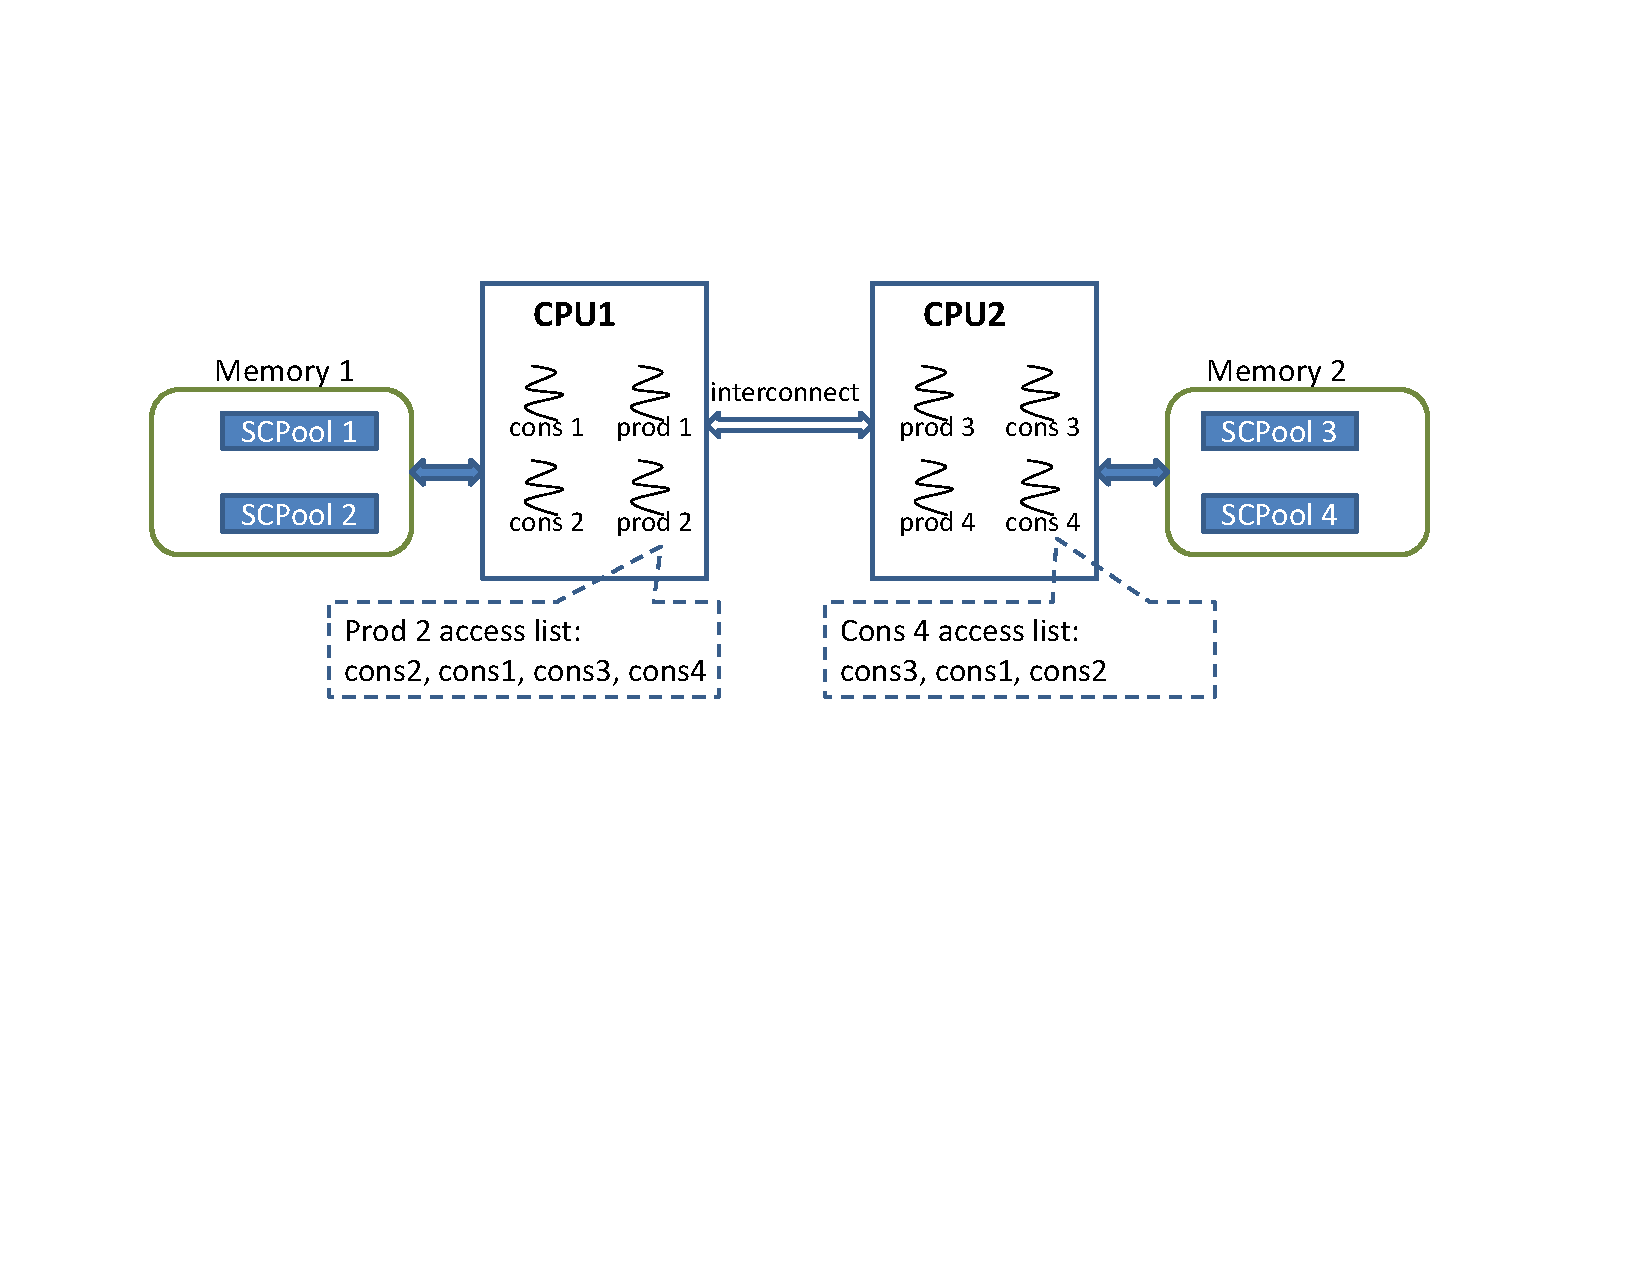
\includegraphics[width=0.7\textwidth]{figures/system-fig}
	\caption{\footnotesize{System overview of the management framework. In the given example the system is composed of two processors that are connected to their own memory banks (NUMA architecture). There are two producers and two consumers running on each processor, the data of each consumer is allocated at the closest available physical memory. A producer $p_i$ has an access list of consumers for task insertion. A consumer $c_i$ has an access list of consumers for task stealing. }}
	\label{fig:system-fig}
\end{figure}

\paragraph {Management policy.}
A management policy is generally defined by the way in which: (1) a producer chooses one of the SCPools to insert a task to, and when it chooses to use produce force; and (2) a consumer decides when to retrieve a task from its own pool and steal tasks from other pools. 
Note that the policy is independent of the underlying SCPool implementation. We believe that it is a subject for engineering optimizations, based on specific workloads and demands.


In the current work, we present a policy that exploits the locality properties of NUMA architectures and is aimed at achieving maximal throughput. If the individual SCPools themselves are lock-free and starvation-free, then our policy preserves these properties at the system level. Our policy is as follows:
\begin{itemize}
	\item {\bf Access lists.} Each process in the system (producer or consumer) is provided with an \emph{access list}, an ordered list of consumers, sorted according to their distance from that process (see Figure~\ref{fig:system-fig}). Intuitively, our policy is to have a producer mostly interact with the closest consumer, while stealing mainly happens inside the same processor node. 
	\item {\bf Producer's policy.} A producer inserting a task first calls the \emph{produce} function of the first SCPool in its access list. Note that a produce operation might fail if the pool is full, (which can be seen as evidence of that the corresponding consumer is overloaded).  In this case, the producer tries to insert the task into other pools, in the order defined by its access list. If all insertions fail, the producer invokes the \emph{produceForce} operation on the closest SCPool, which always succeeds (expanding the pool if needed). 
	\item {\bf Consumer's policy.} A consumer consumes tasks from its own SCPool. If its SCPool is empty, the consumer tries to steal tasks from other pools in the order defined by its access list. 
\end{itemize}



% The inter-pool communication policy is a subject to engineering optimizations and its optimal behavior should probably
% depend on the workload. For the purpose of our evaluation we propose the following approach. 
	% Producer policy. Each producer is provided with the list of all available consumers sorted according to the locality considerations of the given architectures. For example, in case of 
% In order to insert a task a producer first invokes a produce() operation on the closest consumer. If this operation fails, 
% then the closest consumer's pool is full (which could be evidence of an over-load of the given consumer thread) and the producer should 
% try to insert a task to another consumer. If neither consumer ... a producer finally invokes produceForce(), which expands the pool if necessary and always succeeds to insert the task. 
	% Consumer policy. A consumer works in a loop of consuming its own tasks. If the own pool of a consumer is empty, the consumer iterates over all other consumers and tries to steal tasks from there. 



\negspace
\section{Algorithm Description}
\label{sec:algo}
\negspace
In the current section we present the SALSA SCPool. We first show the data structures of SALSA in Section~\ref{alg-structure}, and then present the basic algorithm without stealing support in Section~\ref{alg-overview}. The stealing procedure is described in Section~\ref{alg-stealing}, finally, the role of chunk pools is presented in Section~\ref{alg-pools}.
\negspace
\subsection{SALSA Structure\label{alg-structure}}
\newcounter{alg:non-fifo:lines}
\begin{algo}[!ht]
\caption{SALSA implementation of SCPool: Data Structures.} 
\label{alg:non-fifo-ds}
\scriptsize
\begin{minipage}[t]{0.48\textwidth}
\begin{distribalgo}[1]
\smallskip

\INDENT {{\bf Chunk type}}
	\STATE Task[CHUNK\_SIZE] tasks 
  \STATE int owner \comment {owner's consumer id}
\ENDINDENT

\INDENT {{\bf Node type}}
  \STATE Chunk c; initially $\bot$
  \STATE int idx; initially -1
  \STATE Node next; 
\ENDINDENT

\setcounter{alg:non-fifo:lines}{\value{ALC@line}} % store the line number
\end{distribalgo}
\end{minipage}%
%
\hfill
%
\begin{minipage}[t]{0.48\textwidth}
%
\begin{distribalgo}[1]
\setcounter{ALC@line}{\value{alg:non-fifo:lines}}
\smallskip

\INDENT {{\bf SALSA per consumer data structure}:}
  \STATE int consumerId
  \STATE List\tup{Node}[] chunkLists \comment {one list per producer + extra list for stealing (every list is single-writer multi-reader)} 
  \STATE Queue\tup{Chunk} chunkPool \comment {pool of spare chunks}
  \STATE Node currentNode, initially $\bot$ \comment {current node to work with} 
\ENDINDENT

\setcounter{alg:non-fifo:lines}{\value{ALC@line}}
\end{distribalgo}
\end{minipage}
\end{algo}


\begin{figure}[htb]
	\centering
	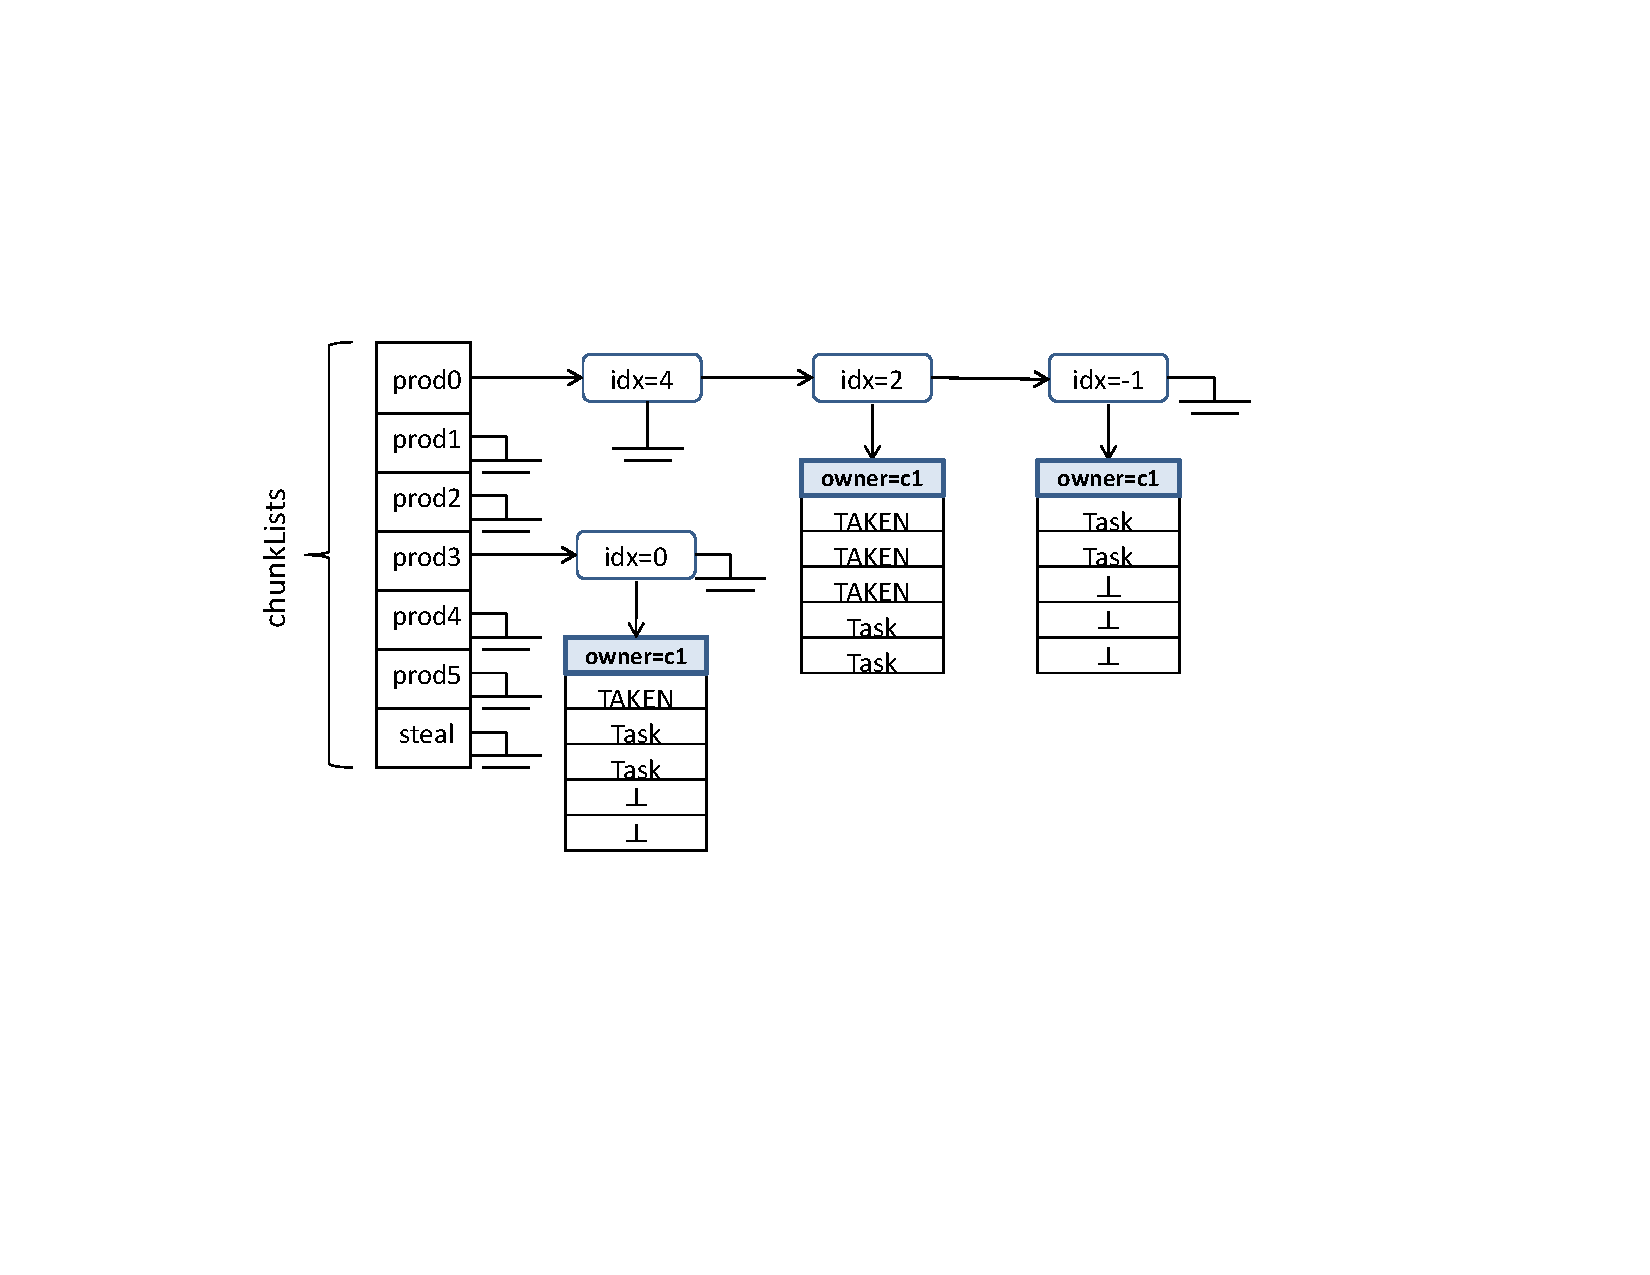
\includegraphics[height=0.3\textwidth]{figures/salsa-struct}
	\caption{
	    \footnotesize{Chunk lists in SALSA single consumer pool implementation. Tasks are kept in chunks, which are 
	    organized in per-producer lists; an additional list is reserved for stealing. Each list can be modified 
	    by the corresponding producer only. The only process that is allowed to retrieve tasks from a chunk is 
	    the owner of that chunk (defined by the ownership flag). A Node's index corresponds to the latest task taken from the chunk
	    or the task that is about to be taken by the current chunk owner. 
	    }}
	\label{fig:salsa-struct}
\end{figure}

We describe the implementation of a SALSA SCPool of some consumer $c_i$.
Its data structures are described in Algorithm~\ref{alg:non-fifo-ds} and partially depicted in Figure~\ref{fig:salsa-struct}. The tasks inserted to SALSA are kept in chunks, which are organized in per-producer chunk lists. Only the producer mapped to a given list can insert a task to any chunk in that list. Every chunk is owned by a single consumer whose id is kept in the \emph{owner} field of the chunk.
The owner is the only process that is allowed to take tasks from the chunk; if another process wants to take a task from the chunk, it should first steal the chunk and change its ownership. The owner of a chunk
residing at $c_i$'s SCPool is $c_i$ itself, unless that chunk is being stolen. A task entry in a chunk is used at most once. It holds the value $\bot$ initially, and TAKEN after the task it held has been consumed.

The per-producer chunk lists are kept in the array \emph{chunkLists} (see Figure~\ref{fig:salsa-struct}), where \emph{chunkLists[j]} keeps a list of chunks with tasks inserted by producer $p_j$. In addition, the array has a special entry \emph{chunkLists[steal]}, holding chunks stolen by $c_i$. Every list has a single writer who can modify the list structure (add or remove nodes), \emph{chunkLists[j]} can be modified only by the producer $p_j$, while the list \emph{chunkLists[steal]} can be modified only by the SCPool's owner $c_i$. Specifically, a consumed node (whose chunk was removed by the consumer) is lazily reclaimed and removed by the list's owner (typically a producer). For brevity, this is omitted from the pseudo-code bellow. Having a single writer allows us to implement the lists without synchronization primitives, similarly to the single-writer linked-list in~\cite{Michael:2004:HPS:987524.987595}.

In addition to the chunk pointer, each node keeps the index of the latest taken task. As we show in Section~\ref{alg-stealing}, this index plays a crucial role in chunk stealing. Safe memory reclamation is provided by using hazard pointers~\cite{Michael:2004:HPS:987524.987595} both for nodes and for chunks.

The free (reclaimed) chunks in SALSA are kept inside the SCPools in \emph{chunkPool}, a lock-free queue~\cite{Michael:1996:SFP:248052.248106}. These pools serve two purposes. First, they enable efficient memory reuse. Second, as we show in Section~\ref{alg-pools}, managing per-consumer chunk pools is good for load balancing. 
\negspace
\subsection{Basic Algorithm\label{alg-overview}}




The local variables and algorithms of the producer appear in
Algorithm~\ref{alg:producer-non-fifo}. The producer's code is fairly simple, the producer first
attempt to add tasks to the chunks it previously used, if this is the first produce action or the
previous chunk was already filled, the producer will attempt to take a chunk from the chunk pool and
add it to its list on the pool of the given consumer. If the pool is empty the operation will fail
with a FULL message, if produceForce was called the operation will not fail, instead a new chunk
will be allocated. 


\negspace
\subsection{Stealing\label{alg-stealing}}
The stealing algorithm is presented in a function {\bf steal()} in Algorithm~\ref{alg:non-fifo}. 
We refer to the stealing consumer as $c_s$, the victim process whose chunk is being stolen is called $c_v$, and the stolen chunk is referred to as $ch$.

The idea is to turn $c_s$ to the exclusive consumer of $ch$, such that $s_c$ will be able to take tasks from the chunk without synchronization. 
In order to do that, $c_s$ changes the ownership of $ch$ (line~\ref{alg:line:chown}) and removes the chunk from the list of $c_v$ (line~\ref{alg:line:remove-chunk}). 
Once $c_v$ notices the change in the ownership it stops taking tasks from $ch$ (lines~\ref{alg:lines:stolen-chunk-end}--\ref{alg:lines:stolen-chunk-begin}). 

When the {\bf steal()} operation of $c_s$ occurs simultaneously with the {\bf takeTask()} operation of $c_v$, both $c_s$ and $c_v$ might try to retrieve the same task. Hence, $c_v$ notifies potential stealers of the task it is about to take by incrementing the \emph{idx} value of the $ch$'s node (line~\ref{alg:lines:ind-inc}). This value is later read by $c_s$ in line~\ref{alg:line:copy-prev-node} when creating a copy of $ch$'s node.

%Consider, for example, a scenario in which the $idx$ value is incremented from $10$ to $11$ during $c_v$'s {\bf takeTask()} operation.
Consider, for example, a scenario in which the $idx$ is incremented by $c_v$ from $10$ to $11$. 
If $c_v$ checks the ownership before it is changed by $c_s$, then $c_v$ takes the task at $11$ without synchronization (see line~\ref{alg:lines:fast-path}). Therefore, $c_s$ is never allowed to take a task pointed by \emph{idx}, and hence $c_v$ has to take the task at $11$ even if it observes the ownership change. 
After taking the chunk, $c_s$ will eventually try to take a task pointed by $idx+1$. However, if $c_s$ read $idx$ before it was incremented by $c_v$, $c_s$ might think that the value of $idx+1$ is $11$. In this case, both $c_s$ and $c_v$ will try to retrieve the task at $11$, hence both should use CAS operation in order to retrieve a task: line~\ref{alg:line:cas-steal} for $c_s$ and line~\ref{alg:line:cas-consumer} for $c_v$. 

The above algorithm works correctly as long as the stealing consumer can observe the node with the updated index value. 
This might not be a case if the same chunk is concurrently stolen by another consumer because the \emph{idx} of the original node would be obsolete. 
In order to prevent this situation, stealing a chunk from the pool of consumer $c_v$ is allowed only if $c_v$ is the owner of this chunk (line~\ref{alg:line:chown}). 

A naive way for $c_s$ to steal the chunk from $c_v$ would be first to change the ownership and then to move the chunk to the steal list. However, that would make our algorithm blocking because there exists a time that the chunk is unaccessible via the lists of $c_s$ and yet $c_s$ is its owner. In this case, as we explained above, the chunk cannot be stolen, which prevents taking the tasks from this chunk by other consumers. Therefore, our solution is to first add the original node to the steal list of $c_s$, change the ownership, and only then to replace the original node with a new node (lines~\ref{alg:line:resteal-begin}--\ref{alg:line:resteal-end}). 
 

% change the ownership (the consumer will check the ownership change)
% what about the first task retrieval? (the description includes the explanation about idx+1)
% what about concurrent stealing? (I want to see the updated idx value, the updated idx value is kept at node, hence I need to steal from the owner only)
% what about non-blocking properties? (want to allow others to always find a task...) 






% \paragraph{Stealing the chunk.} Before stealing a chunk, $c_1$ has to make sure $c_2$ will not take any more tasks from that chunk, so the $c_1$ may later take tasks with no need for synchronization. To achieve this $c_1$ must change the owner field of the chunk. Changing the ownership will prevent $c_2$ from taking tasks as a consumer always checks that he is the owner of the chunk before taking tasks. 
% 
% Before changing the ownership we must relate to two issues: (1) Stealing a chunk from the pool of consumer $c_2$ is allowed only if $c_2$ is the owner of the chunk that we steal, this is needed so it is guaranteed that $c_2$ reads the latest value of the idx, which is only found in the owner's node. (2) We want that other consumers would be able to steal the chunk during the process, so that the algorithm will stay lock-free. 
% 
% For those two reasons we must make the chunk accessible via $c_1$'s pool before changing ownership. However, we cannot simply add a new node to $c_1$'s steal list, as that node's idx field will not be updated if $c_2$ changes his idx field. Therefore, before changing ownership, $c_1$ adds $c_2$'s node to his steal list (Line~\ref{} in Algorithm~\ref{}). Now $c_1$ takes ownership (Line~\ref{}) and creates a new node with the updated idx that will replace the $c_2$'s node (Line~\ref{}), as the original idx may only change by one pending operation at most. Finally $c_1$ changes $c_2$'s node to point to NULL (Line~\ref{}) so that this node will not be used and will be lazily removed.
% 
% \paragraph{Taking the first task.} After the $c_1$ stole the chunk, he must attempt to take a task, so Property~\ref{steal-progress-property} will hold. $c_1$ will try to take the task at $idx+1$, however, this task may be also taken by $c_2$ if he started a consume operation before $c_1$ completed the node transfer. This is why $c_1$ must use a CAS operation to take this node (Line~\ref{}). $c_2$ must also attempt to take this node (Line~\ref{}) even if he noticed the ownership change, since he does not know if $c_1$ read the idx value before or after $c_2$ increased it Line~\ref{}.

% \vspace{5mm}\noindent
% We claim that the steal operation hold Property~\ref{steal-progress-property}. In line~\ref{} a chunk with at least one task is taken, therefore there is a task at $idx+1$. if $idx$ is updated during the stealing operation it means that the original consumer is taking that task and therefore the property holds. Otherwise, either the CAS in line~\ref{} failed and another consumer successfully stole the chunk and will return a task, or the current producer will reach line~\ref{}. In this line the CAS will be executed if the task wasn't already taken, and since either the stealing consumer or the original consumer will succeed performing the CAS.
\negspace
\subsection{Chunk Pools\label{alg-pools}}
As described in Section~\ref{alg-structure}, each consumer keeps a pool of free chunks.
When a producer needs a new chunk for adding a task to consumer $c_i$, it tries to get a chunk from $c_i$'s chunk pool -- if no free chunks are available, the {\bf produce()} operation fails.

As described in Section~\ref{sec:system}, our system-wide policy defines that if an insertion operation fails, then the producer tries to insert a task to other pools. Thus, the producer avoids adding tasks to overloaded consumers, which in turn decreases the amount of costly steal operations. 

Another SALSA property is that a chunk is returned to the pool of a consumer that retrieves the latest task of this chunk. 
Therefore, the size of the chunk pool of consumer $c_i$ is proportional to the rate of $c_i$'s task consumption.
This property is especially appealing for heterogeneous systems -- a faster consumer $c_i$ ", (e.g., one running on a stronger or less loaded core), will have a larger chunk pool, and so more {\bf produce()} operations will insert tasks to $c_i$, automatically balancing the overall system load. 

\negspace
\section{Correctness}
\label{sec:correctness}
\begin{figure}[htb]
	\centering
	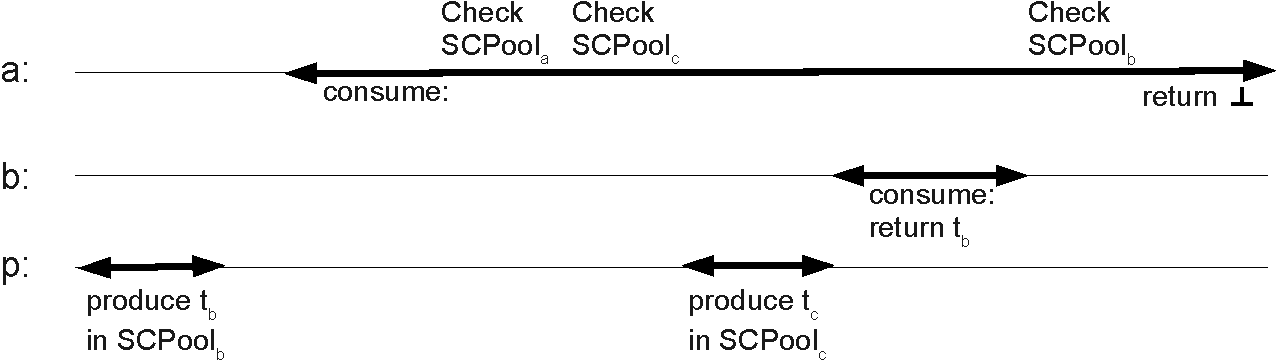
\includegraphics[width=0.7\textwidth]{figures/linearizability-example}
	\caption{\footnotesize{In this scenario $a$, $b$ and $c$ are the only consumers in the system and $p$ is the only producer. Above is a description of the following execution were $a$ trying to get a task: consumer $a$ fails to take a task from its own pool, and starts looking for chunks to steal in other pools. Assume that at this time there is a single non-empty chunk in the system, which is in $b$'s pool. Assume further that $a$ checks $c$'s pool before $b$'s pool and sees that it is empty. At this point a producer adds a task to $c$'s pool and then $b$ takes the last task from its pool before $a$ checks it. Thus, $a$ finds $b$'s pool to be empty, and returns $\bot$. There is no way to linearize this execution, because throughout the execution of the $a$'s operation, the system contained a task.}}
	\label{fig:linearizability-example}
\end{figure}

\paragraph{linearizability}
The algorithm as described in the previous sections is trivially wait-free as all operations of the SALSA pool always return, and the framework only calls a bounded number of those operations. However, this algorithm does not implement a linearizable task pool because an operation may return $\bot$ even when the pool is not empty. 

There are two possible reasons why a consumer may incorrectly return $\bot$. First, the consumer may ``miss'' one task added during its traversal, and another removed during the same traversal. Second, a consumer may miss a task in case a chunk is moved from one pool to another due to stealing. In order to identify these two cases, we add to each pool special counter \emph{emptyCount}, which is increased every time a chunk is reclaimed or stolen (i.e., every time a chunk is removed from the pool).
See the example in Figure~\ref{fig:linearizability-example}.

we now describe a way to make our algorithm linearizable which makes it only lock-free. 
We change the framework of section \ref{sec:system} so that a new function {\bf checkEmpty()} is called whenever a consumer fails to retrieve tasks from its pool and all other pools. This function ensures that $\bot$ is returned only if there is a time when there are no tasks in the system. If {\bf checkEmpty()} finds that the pool is not empty, the consumer restarts its operation. The {\bf checkEmpty()} function works as follows: the consumer traverses all the chunk lists of all SALSA pools in the system, to make sure that no tasks are present. After checking a pool, it reads its value of the \emph{emptyCount}. The consumer repeats this traversal $|consumers|$ times, where in all traversals except the first, it checks that the \emph{emptyCount} value is equal to the value it saw in the first traversal, i.e., that no chunks were moved during the traversal. The reason the consumer makes $|consumers|$ traversals is that other consumers may already stole or removed chunks but did not yet change \emph{emptyCount} and therefore their operations were not detected by the consumer. Since there may be up to $|consumers-1|$ pending operations by other consumers, it is guaranteed that after $|consumers|$ traversals in which no chunks were seen and the \emph{emptyCount} did not change, in one of the traversals the system contains no tasks, and therefore it is safe to return $\bot$. This method is similar to the one used in Concurrent Bags~\cite{Sundell:2011:LAC:1989493.1989550}. However, while our method requires a single fetch-and-increment operation per-steal and per-chunk, their operation requires an additional write on every produce operation, and a CAS operation for every empty chunk encountered in the traversal.

\paragraph{Lock-freedom}
This approach does not guarantee that a consumer will finish its operation. For example, in case the consumer's pool is empty, and its steal operation always fails, even when the system contains chunks, this consumer does not make progress. Nevertheless, the system is lock-free, i.e., there always exists some consumer that makes progress. Lock-freedom follows immediately from the following claim:


\begin{claim}
\label{claim:lock-free}
If a consumer fails in $c$ steal attempts from non-empty pools, where $c$ is the number of consumers in the system, then it is guaranteed that at least one consumer in the system returns a task during that time. 
\end{claim}
The proof for this claim is described in Appendix \ref{appendix:lock-freedom}.
\negspace
\section{Evaluation}
\label{sec:evaluation}
In this section we evaluate the performance of our work-stealing framework built upon SALSA pools. 
We describe the experiment setup in Section~\ref{sec:exp-setup}, we show the overall system performance in Section~\ref{sec:eval-performance} and study the influence of various SALSA techniques in Section~\ref{sec:eval-techniques}.

\subsection {Experiment Setup}
\label{sec:exp-setup}
The implementation of the work-stealing framework used in our evaluation does not include the linearizability mechanism described in~\ref{sec:correctness}. We believe that this mechanism has negligible effect on performance; moreover, in our experiment they would not have been invoked because the pool is never empty. We compare the following task pool implementations:
\begin {itemize}
\item
{\bf SALSA} -- our work-stealing framework with SCPools implemented by SALSA.
\item
{\bf SALSA+CAS} -- our work-stealing framework with SCPools implemented by a simplistic SALSA variation, in which every {\bf consume()} and {\bf steal()} operation tries to take a single task using CAS. In essence, SALSA+CAS removes the effects of SALSA's low-synchronization fast-path and per-chunk stealing. 
Note that disabling per-chunk stealing in SALSA annuls the idea of chunk ownership, hence, disables its low-synchronization fast-path as well. 
\item
{\bf ConcBag} -- an algorithm similar to the lock-free Concurrent Bags algorithm~\cite{Sundell:2011:LAC:1989493.1989550}. 
It is worth noting that the original algorithm was optimized for the scenario where the same process is both a producer and a consumer (in essence producing tasks to itself), which we do not consider in this paper; in our system no thread acts as both a producer and a consumer, therefore every consume operation steals a task from some producer.
We did not have access to the original code, and therefore reimplemented the algorithm in our framework. Our implementation is faithful to the algorithm in the paper, except in using a simpler and faster underlined linked list algorithm. All engineering decisions were made to maximize performance. 
\item
{\bf WS-MSQ} -- our work-stealing framework with SCPools implemented by Michael-Scott non-blocking queue~\cite{Michael:1996:SFP:248052.248106}. Both {\bf consume()} and {\bf steal()} operations invoke the {\bf dequeue()} function. 
\item
{\bf WS-LIFO} -- our work-stealing framework with SCPool implemented by Michael's LIFO stack~\cite{Michael:2004:HPS:987524.987595}. 
\end {itemize} 

We did not experiment with additional FIFO and LIFO queue implementations, because, as shown in~\cite{Sundell:2011:LAC:1989493.1989550}, their performance is of the same order of magnitude as the Michael-Scott queue. 
Similarly, we did not evaluate {CAF\'E}\cite{Basin:2011:CST:2075029.2075087} pools because their performance is similar to that of WS-MSQ~\cite{Basin:Thesis:2011}, or ED-Pools~\cite{Afek:2010:SPP:1885276.1885295}, which have been shown to scale poorly in multi-processor architectures~\cite{Basin:Thesis:2011,Sundell:2011:LAC:1989493.1989550}. 

All the pools are implemented in C++ and compiled with \texttt{-O2} optimization level. 
In order to minimize scalability issues related to allocations, we use \texttt{jemalloc} allocator~\cite{citeulike:4951109}, which has been shown to be highly scalable in multi-threaded environments\footnote{\url{http://www.facebook.com/notes/facebook-engineering/scalable-memory-allocation-using-jemalloc/480222803919}}.
Unless stated otherwise, chunks of SALSA and SALSA+CAS contain $1000$ tasks, and chunks of ConcBag contain $128$ tasks, which were the respective optimal values for each algorithm (see Appendix \ref{appendix:chunk-size}). 

We use a synthetic benchmark where 1) each producer works in a loop of inserting dummy items; 2) each consumer works in a loop of retrieving dummy items. Each data point shown is an average of $5$ runs, each with a duration of $20$ seconds. 
The tests are run on a dedicated shared memory NUMA server with $8$ Quad Core AMD $2.3$GHz processors and $16$GB of memory attached to each processor. 

\subsection{System Throughput}
\label{sec:eval-performance}

\begin{figure}[htb]
	\centering
  \subfigure [\scriptsize{System throughput -- N producers, N consumers.}] {
    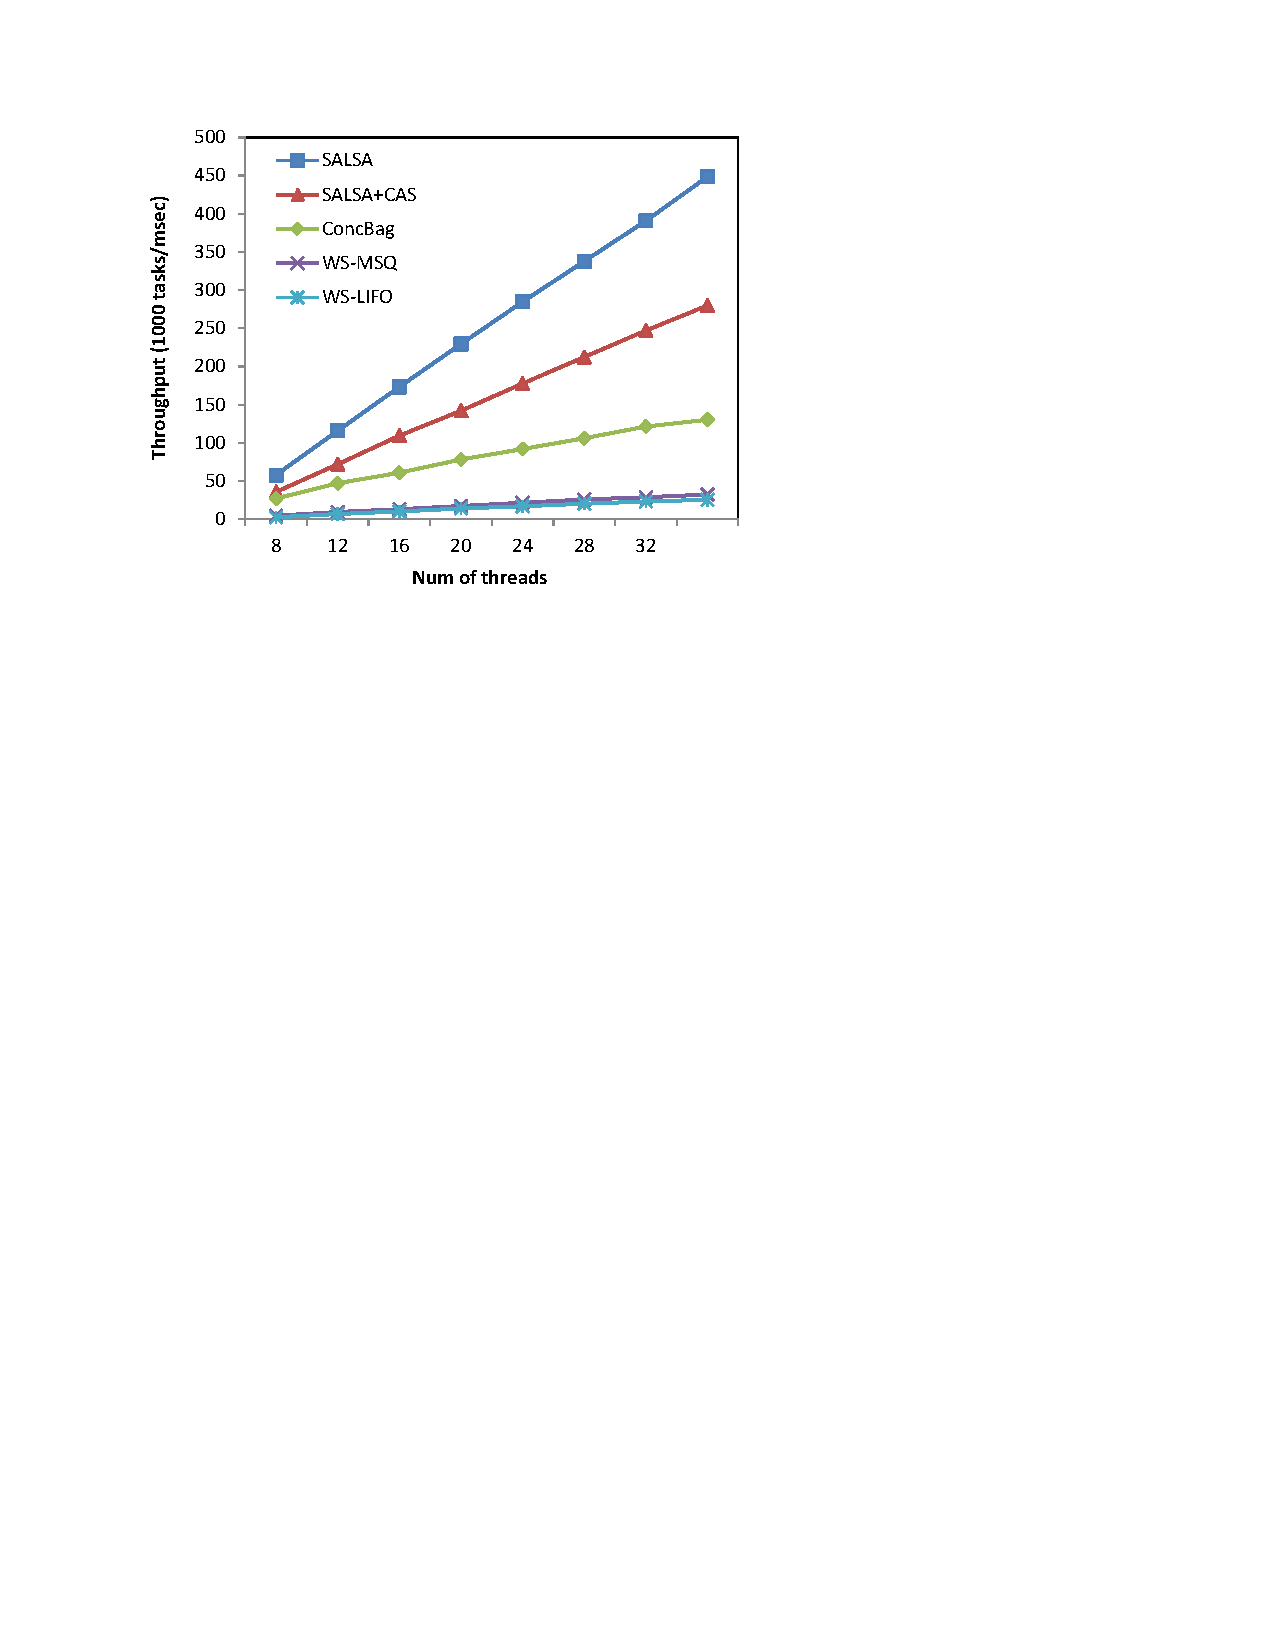
\includegraphics[width=0.45\textwidth]{figures/n-n-throughput}
    \label{fig:n-n-throughput}
  }
  \subfigure [\scriptsize{System throughput -- variable producers-consumers ratio.}] {
    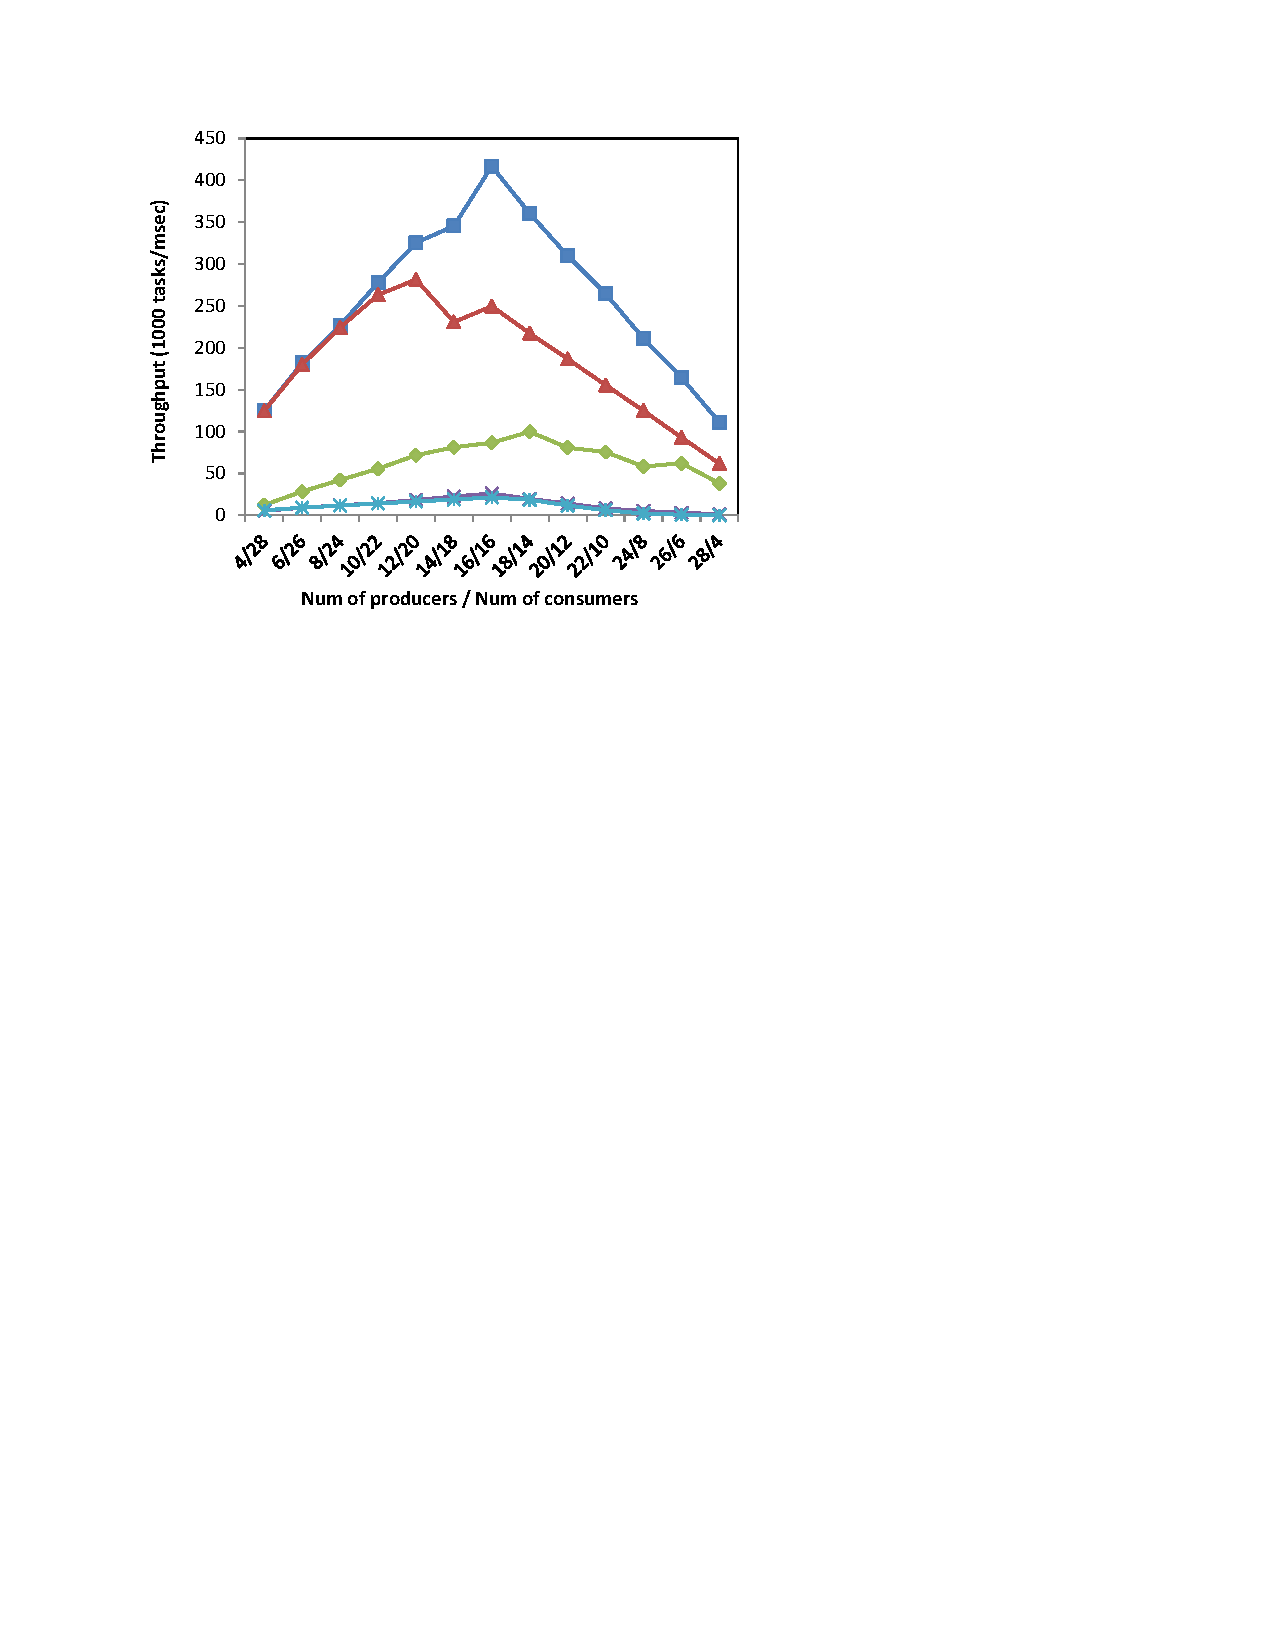
\includegraphics[width=0.45\textwidth]{figures/prod-cons-fig}
    \label{fig:prod-cons-fig}
  }
	\caption{\footnotesize{System throughput for various ratios of producers and consumers. SALSA scales linearly with the number of threads -- in the $16/16$ workload, it is $\times20$ faster than WS-MSQ and WS-LIFO, and more than $\times5$ faster than Concurrent Bags. In tests with equal numbers of producers and consumers, the differences among work-stealing alternatives are mainly explained by the consume operation efficiency, since stealing rate is low and hardly influences performance. In Concurrent Bags every {\bf consume()} operation implies stealing, which causes its sub-linear scalability.
}}
	\label{fig:throughput}
\end{figure}

Figure~\ref{fig:throughput} demonstrates system throughput of the compared algorithms for workloads with various numbers of producers and consumers. 
Figure~\ref{fig:n-n-throughput} shows throughput dynamics when the number of producers is equal to the number of consumers. SALSA \emph{scales linearly} as the number of threads grows to $32$ (the number of physical cores in the system), and it clearly outperforms all other competitors. In the $16/16$ workload, SALSA is $\times20$ faster than WS-MSQ and WS-LIFO, and more than $\times5$ faster than Concurrent Bags. 

We note that the performance trend of ConcBags in our measurements differs from the results presented by Sundell et al.~\cite{Sundell:2011:LAC:1989493.1989550}. 
While in the original paper, their throughput \emph{drops} by a factor of $3$ when the number of threads increases from $4$ to $24$, in our tests, the performance of ConcBags \emph{increases} with the number of threads. The reasons for the better scalability of our implementation compared of the original one can be related to the use of different memory allocators, hardware architectures, and engineering optimizations. %In any case, both implementations provide the performance of tens of thousands of task retrievals in msec for multiple producers and consumers. 

The stealing rate in workloads with equal numbers of producers and consumers remains low; graphs showing these results are omitted due to space limitations. The performance differences are therefore due to the efficiency of the {\bf consume()} operation. 
For example, SALSA is $\times1.7$ faster than SALSA+CAS thanks to the fast-path consumption technique, which does not use strong atomic operations. The impact of CAS operations is fairly modest, however, since they seldom compete.
In contrast, in ConcBags, which is not based on per-consumer pools, every {\bf consume()} operation implies stealing, which causes contention among consumers, leading to sub-linear scalability.

Figure~\ref{fig:prod-cons-fig} shows system throughput of the algorithms for various ratios between producers and consumers. 
Our algorithm achieves maximal throughput for the equal number of producers and consumers because neither of them is a system bottleneck.
SALSA outperforms other alternatives for all possible producer-consumer ratios. 

\begin{figure}[htb]
	\centering
  \subfigure [\scriptsize{System throughput -- 1 Producer, N consumers.}] {
    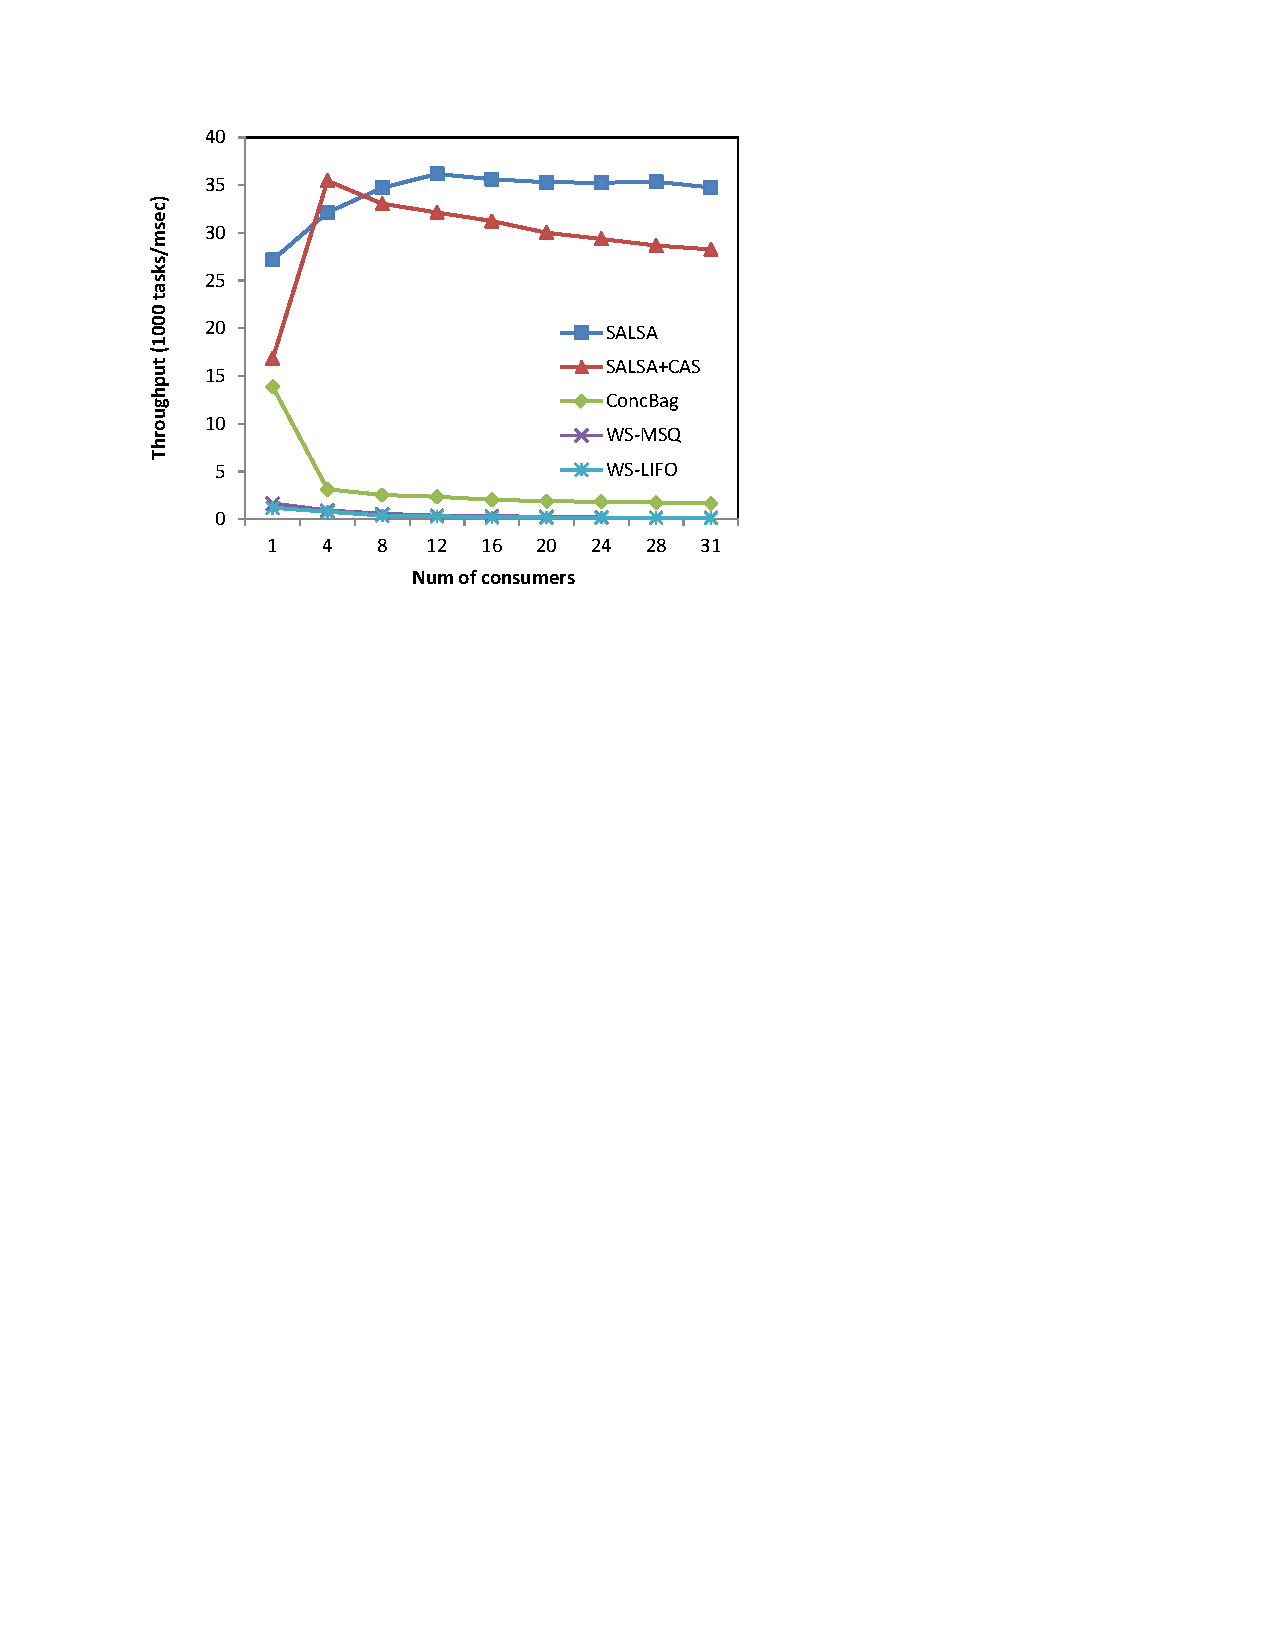
\includegraphics[width=0.45\textwidth]{figures/1-n-throughput}
    \label{fig:1-n-throughput}
  }
  \subfigure [\scriptsize{CAS operations per task retrieval -- 1 Producer, N consumers.}] {
    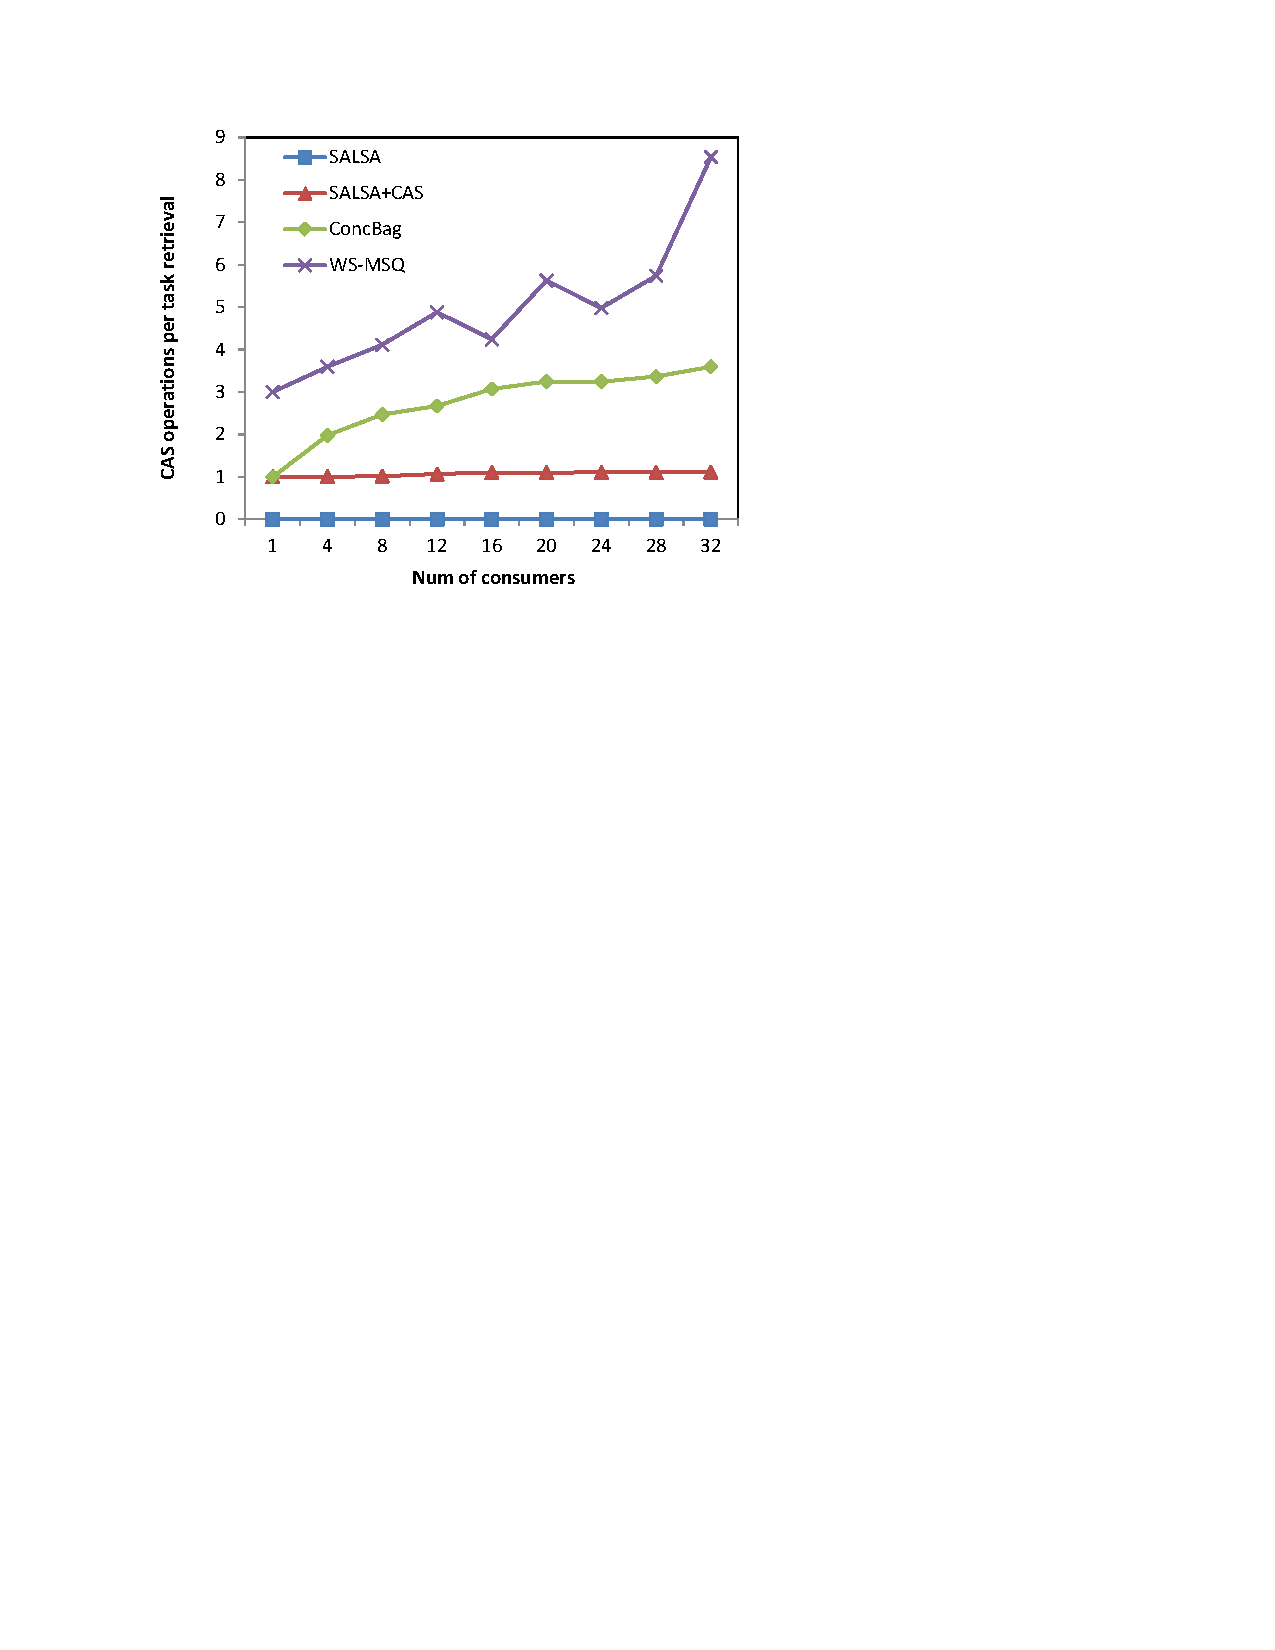
\includegraphics[width=0.45\textwidth]{figures/1-n-cas}
    \label{fig:1-n-cas}
  }
	\caption{\footnotesize{System behavior in workloads with a single producer and multiple consumers. 
	Both SALSA and SALSA+CAS efficiency balance the load in this scenario. The throughput of other algorithms drops by a factor of $10$ due to increased contention among consumers trying to steal tasks from the same pool.}}
	\label{fig:1-n-perf}
\end{figure}

We next evaluate the behavior of the compared pools in scenarios with one producer and many consumers. 
Figure~\ref{fig:1-n-throughput} shows that both SALSA and SALSA+CAS are successful in balancing the load among all consumers with little contention. In contrast, the throughput of other algorithms drops by the factor of $10$ when the number of consumers rises from $1$ to $32$. 
This degradation is caused by the increased contention among consumers that try to steal tasks from the same pool, as evident from Figure~\ref{fig:1-n-cas}, which shows the average number of CAS operations per task transfer (by both producers and consumers). As we shall see in the next section, SALSA+CAS's low contention is achieved thanks to the producer-based balancing described in Section~\ref{alg-pools}. SALSA achieves significantly better throughput thanks to chunk-based stealing.

\subsection{Evaluation of SALSA Techniques}
\label{sec:eval-techniques}
\begin{figure}[htb]
	\centering
  \subfigure [\scriptsize{System throughput -- 1 Producer, N consumers.}] {
    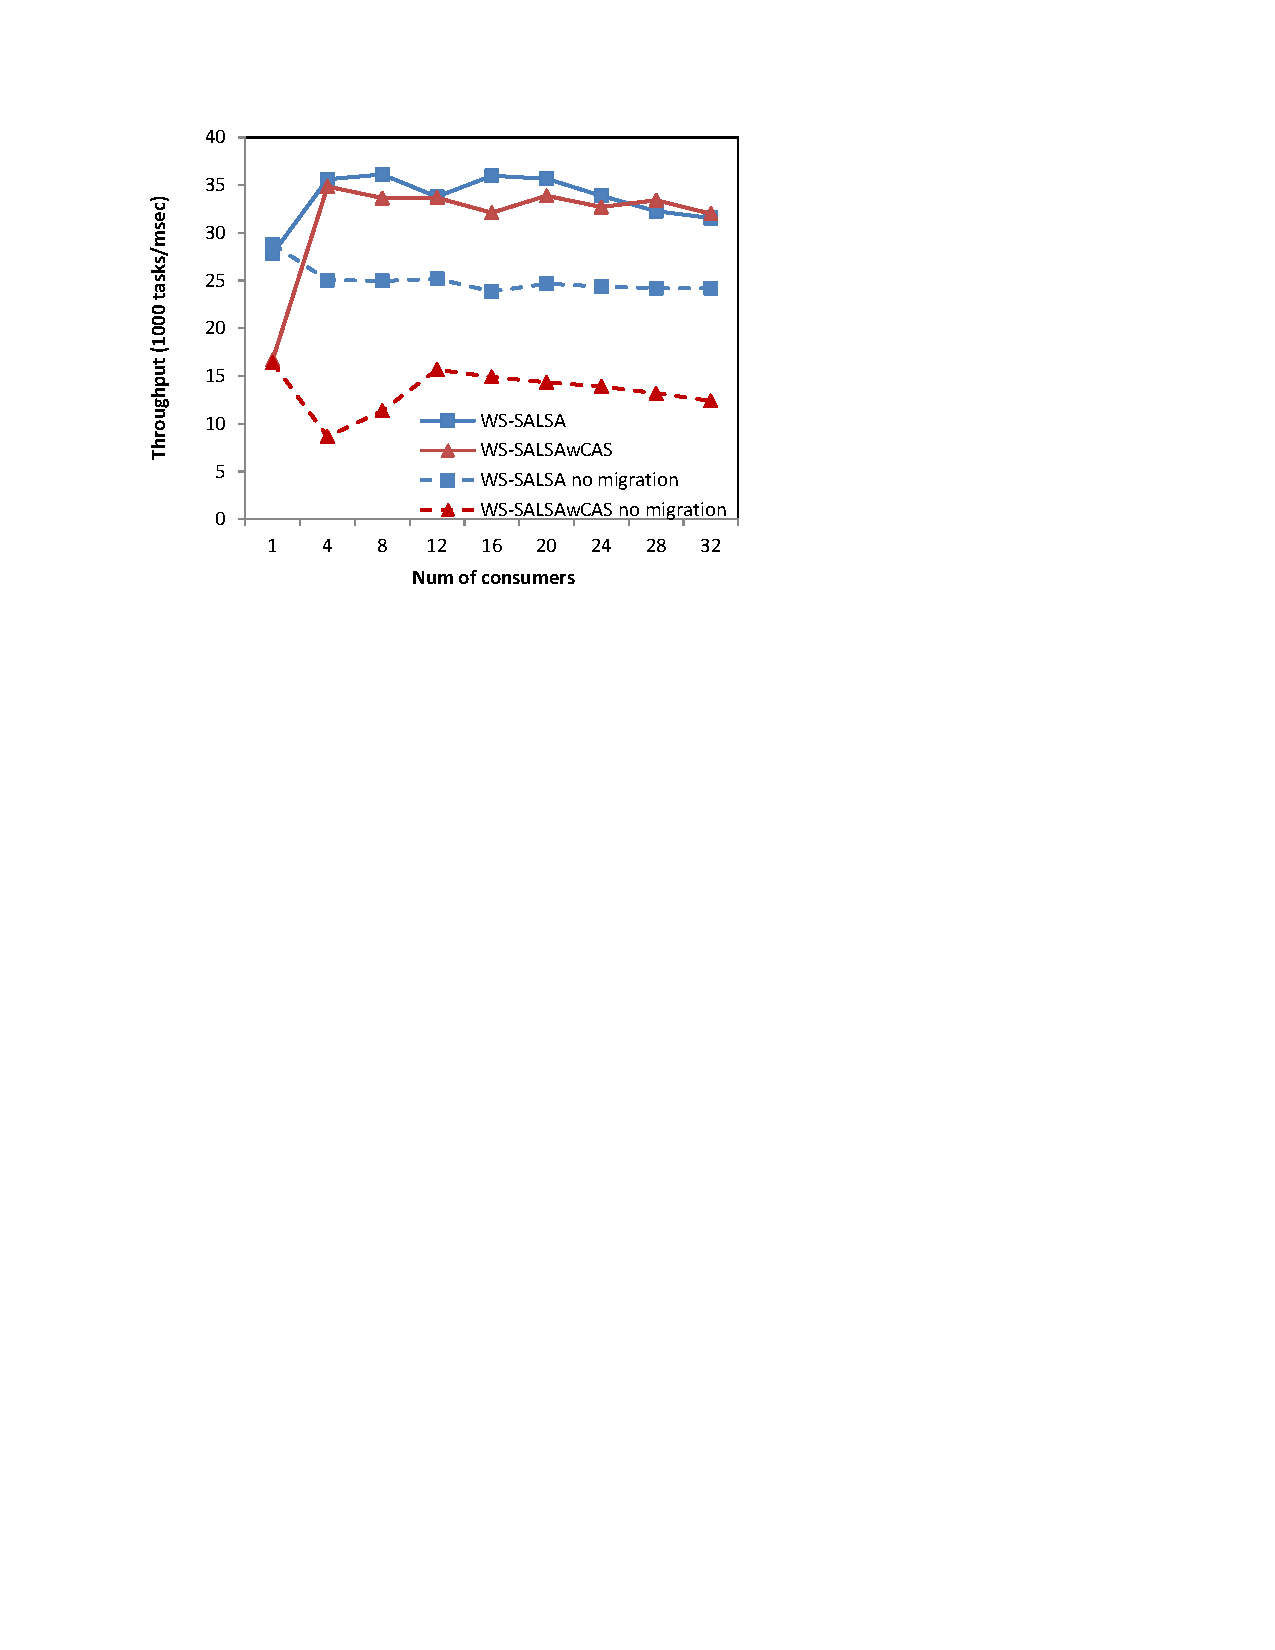
\includegraphics[width=0.45\textwidth]{figures/1-n-salsa}
    \label{fig:1-n-salsa-perf}
  }
  \subfigure [\scriptsize{System throughput as a function of stalled threads ($16/16$ workload). Black dashed lines show the theoretical throughput degradation proportional to the number of stalled threads.}] {
    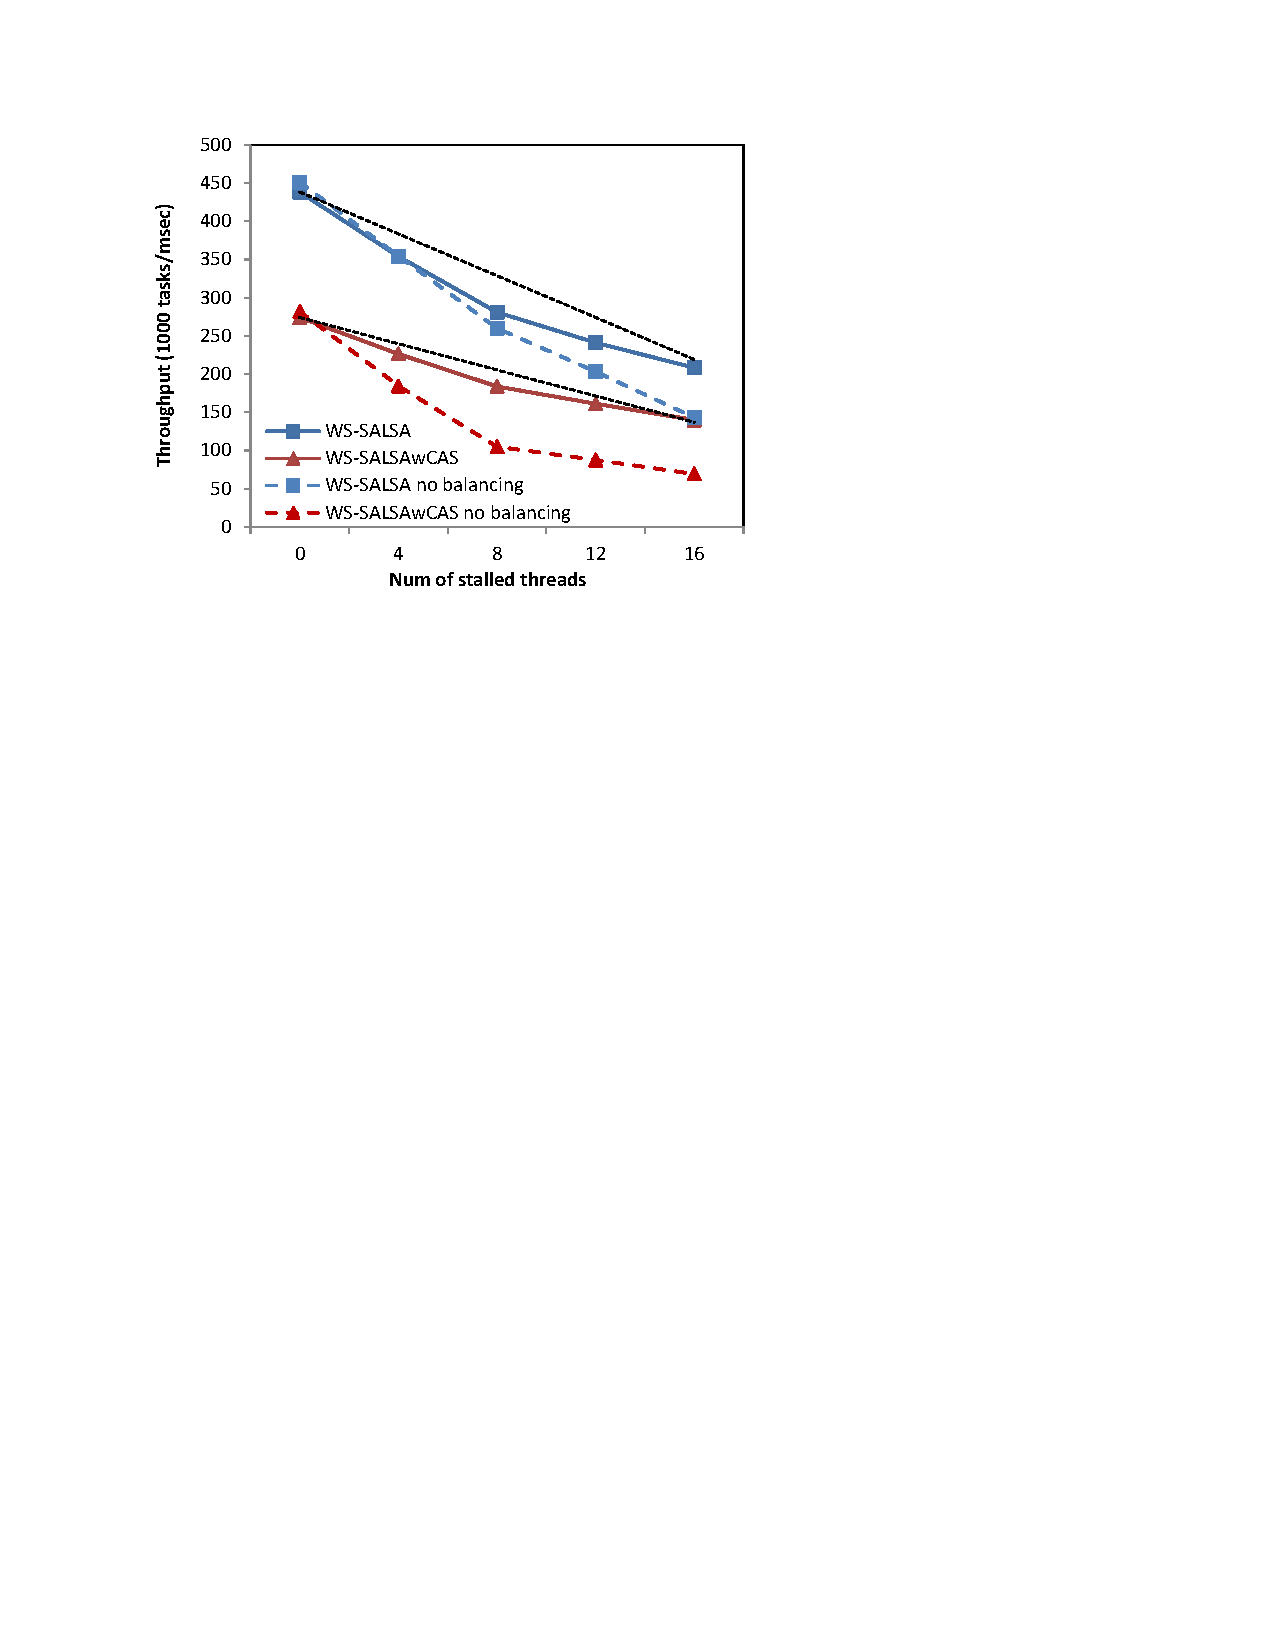
\includegraphics[width=0.45\textwidth]{figures/stalled-threads}
    \label{fig:stalled-threads}
  }
	\caption{\footnotesize{The effects of chunk-based stealing and producer-based balancing on system throughput in imbalanced scenarios. Producer-based balancing contributes to the robustness of the framework by reducing stealing. With no balancing, chunk-based stealing becomes important. }}
	\label{fig:1-n-salsa}
\end{figure}
In this section we study the influence of two of the techniques used in SALSA: 1) chunk-based-stealing with a low-synchronization fast path (Section~\ref{alg-stealing}), and 2) producer-based balancing (Section~\ref{alg-pools}). 
To this end, we compare SALSA and SALSA+CAS both with and without producer-based balancing (in the latter a producer always inserts tasks to the same consumer's pool).

Figure~\ref{fig:1-n-salsa-perf} depicts the behavior of the four alternatives in single producer / multiple consumers workloads. 
We see that producer-based balancing is instrumental in redistribute the load: neither SALSA nor SALSA+CAS suffers any degradation as the load increases. 
When producer-based balancing is disabled, stealing becomes prevalent, and hence the stealing granularity becomes more important: 
SALSA's chunk based stealing clearly outperforms the na\"{i}ve task-based approach of SALSA+CAS. 

Figure~\ref{fig:stalled-threads} considers the case where an equal number of producer and consumer threads are stalled in $16/16$ workload (e.g., if $4$ threads are stalled then there are $2$ paused producers and $2$ paused consumers). This simulates the scenario of an overloaded machine in which some threads can be starved for long periods of time, or a scenario where some threads are busy running excessively long tasks. 
The stalled threads are chosen so that the default producers of the frozen consumers are not stalled, which leads to imbalance in the number of tasks among the SALSA pools. 
Reducing the number of participating threads inherently degrades performance; the black dashed lines indicate the theoretical performance degradation in proportion to the number of stalled threads.
The graphs demonstrate that producer-based balancing contributes to the robustness of the framework, and allows both SALSA variants to achieve performance close to that of the theoretical bound.

When producer-based balancing is disabled, a high stealing rate is inevitable, which causes a severe throughput degradation.

%
%\begin{wrapfigure}{r}{0.47\textwidth}
%  \vspace{-20pt}
%  \begin{center}
%    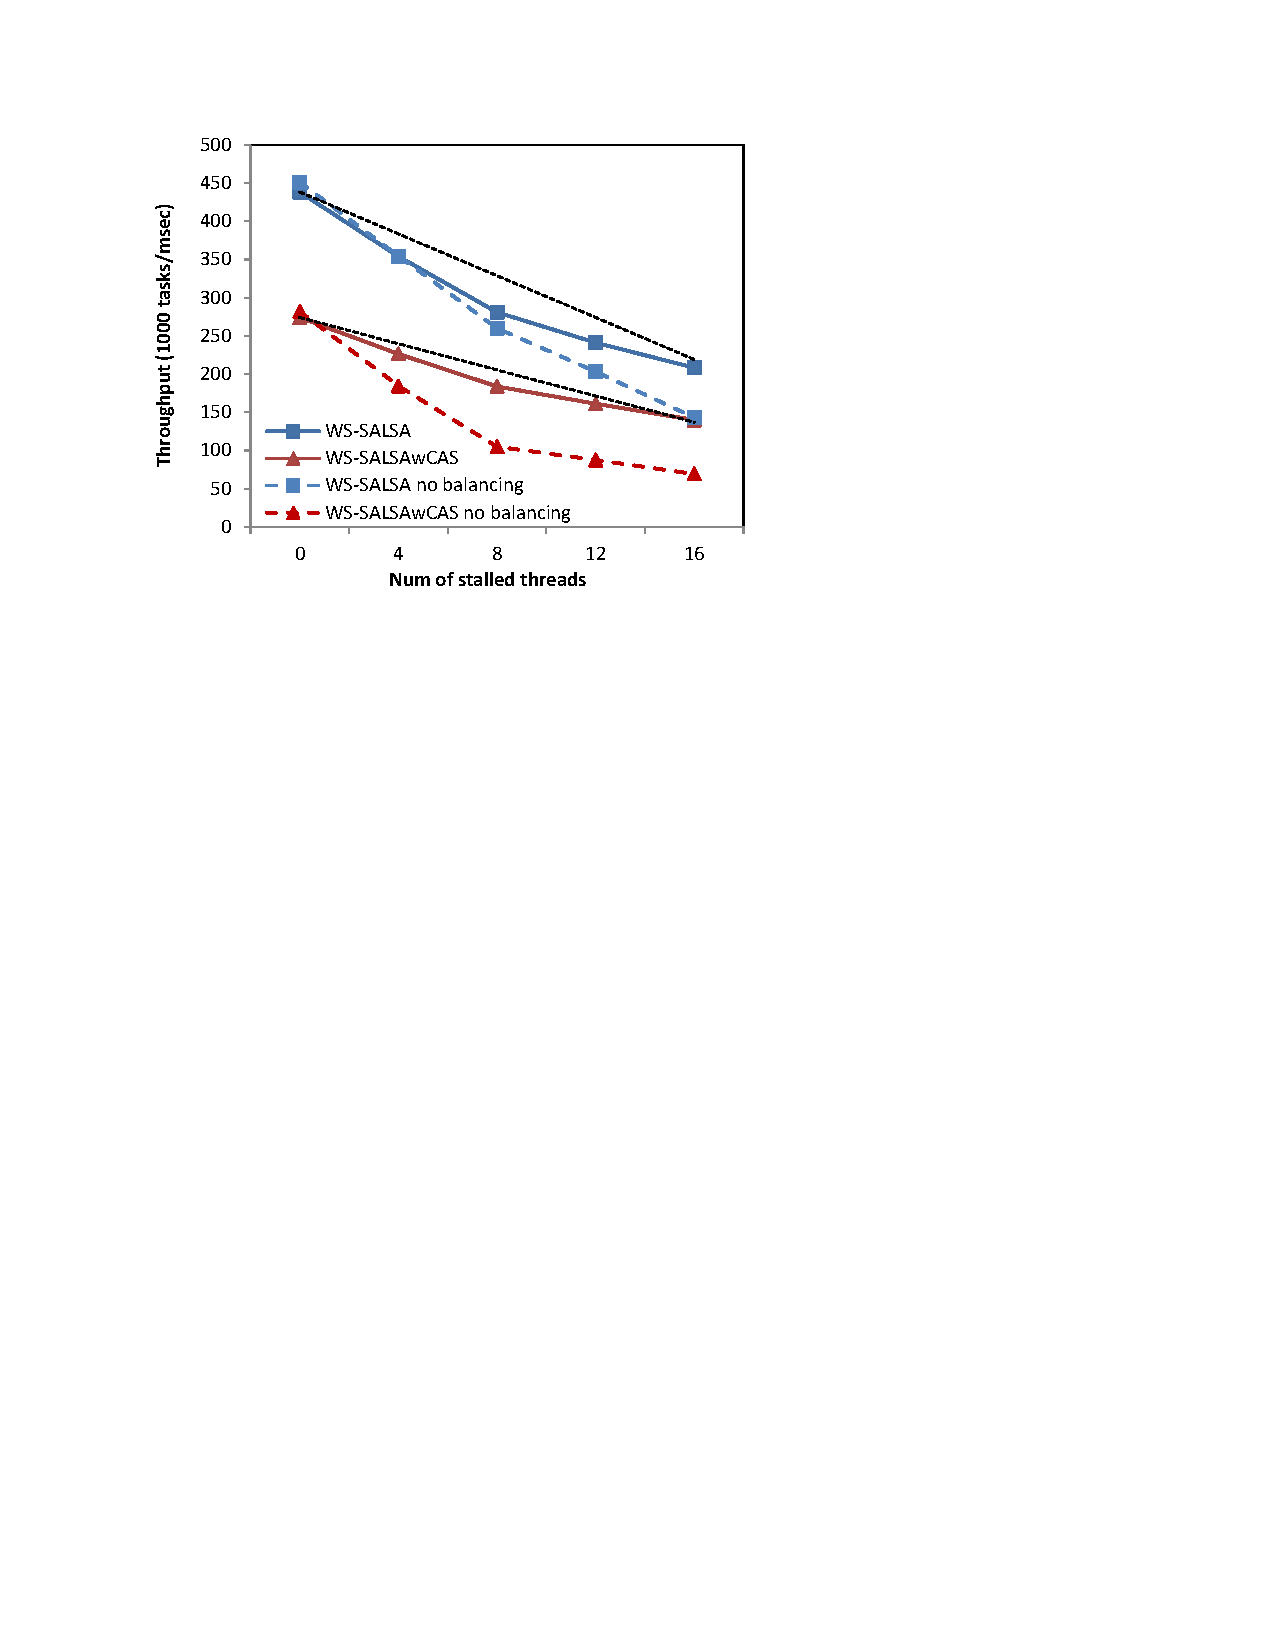
\includegraphics[width=0.45\textwidth]{figures/stalled-threads}
%  \end{center}
%  \vspace{-20pt}
%  \caption{\footnotesize{System throughput in a system with $16$ producers and $16$ consumers as a function of the number of stalled threads.}}
%  \vspace{-10pt}
%  \label{fig:stalled-threads}
%\end{wrapfigure}
%
%%
%%
%%\begin{figure}[htb]
%%	\centering
%%	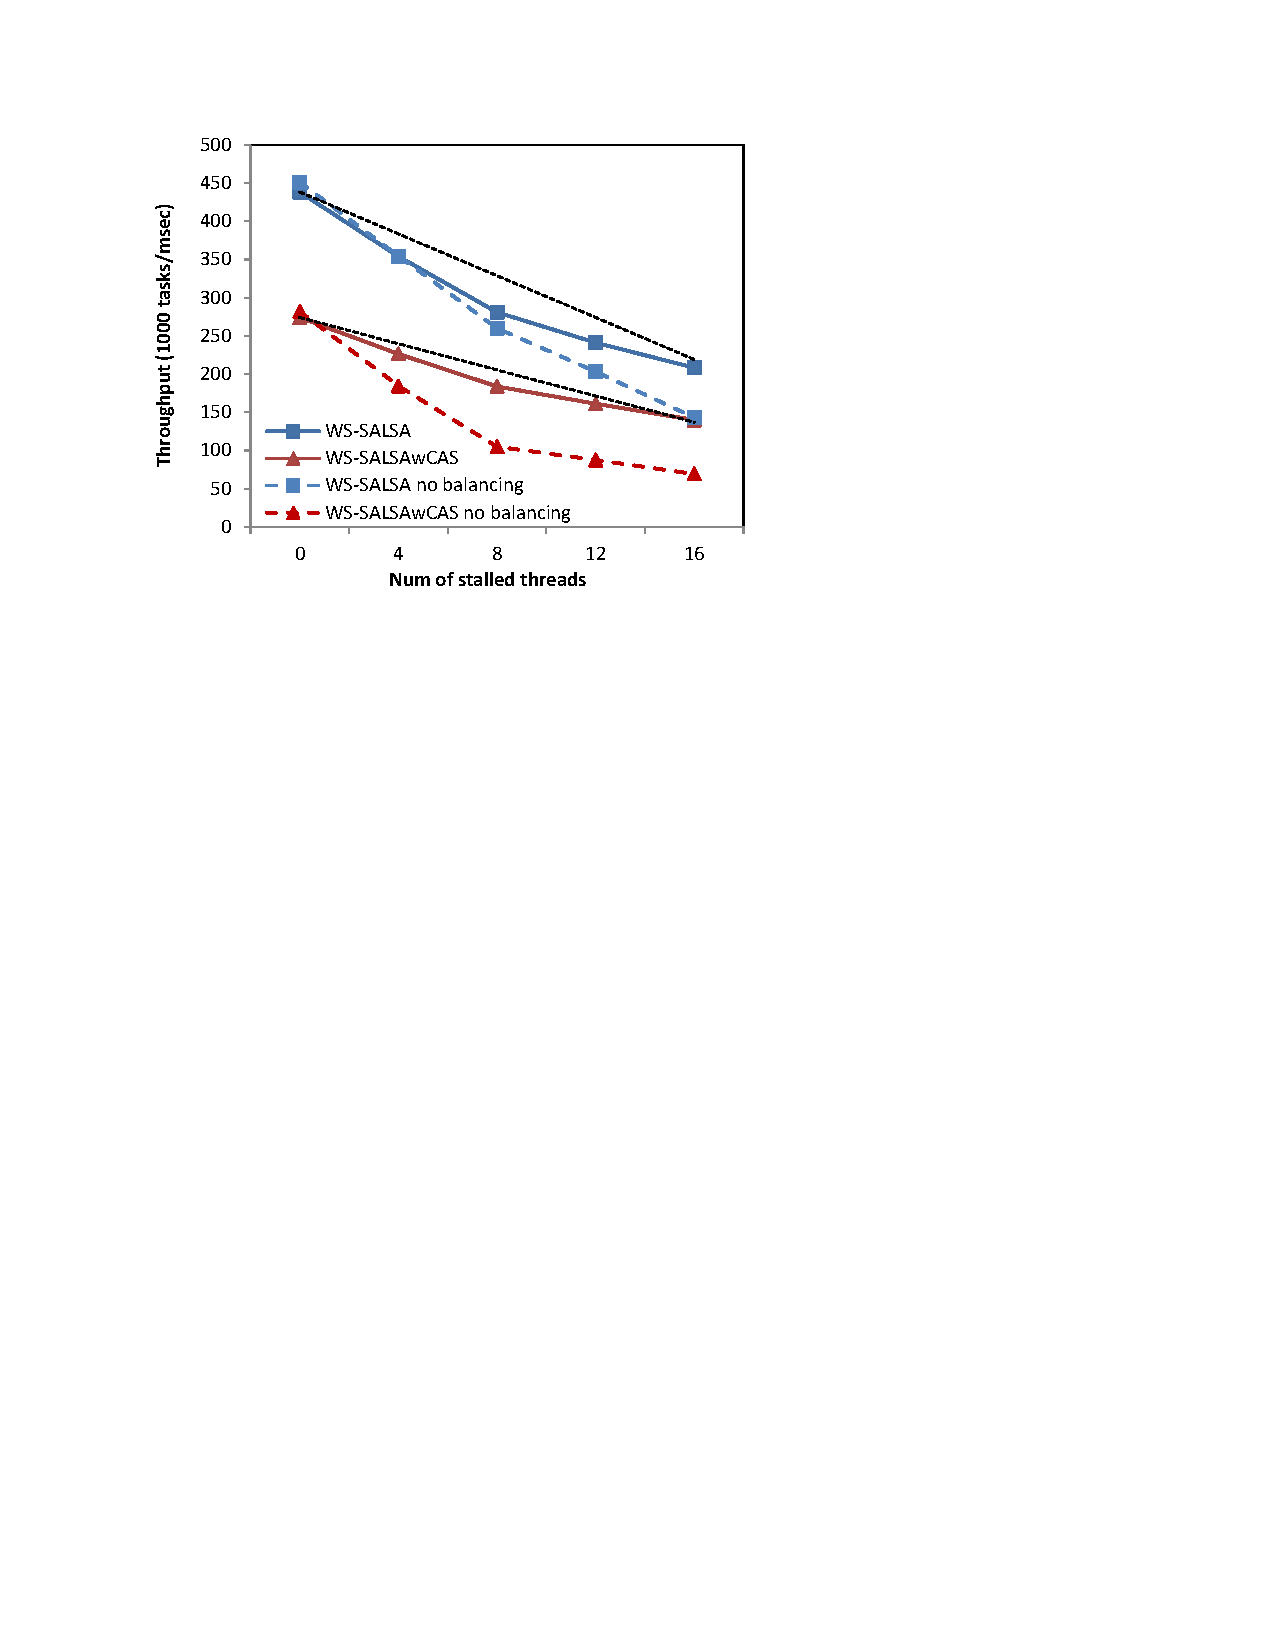
\includegraphics[width=0.45\textwidth]{figures/stalled-threads}
%%  \caption{\footnotesize{System throughput for different number of stalled threads (N/N workload). }}
%%	\label{fig:stalled-threads}
%%\end{figure}
%
%producer migration -- robustness against unpredictable stalls
%
%\begin{figure}[htb]
%	\centering
%	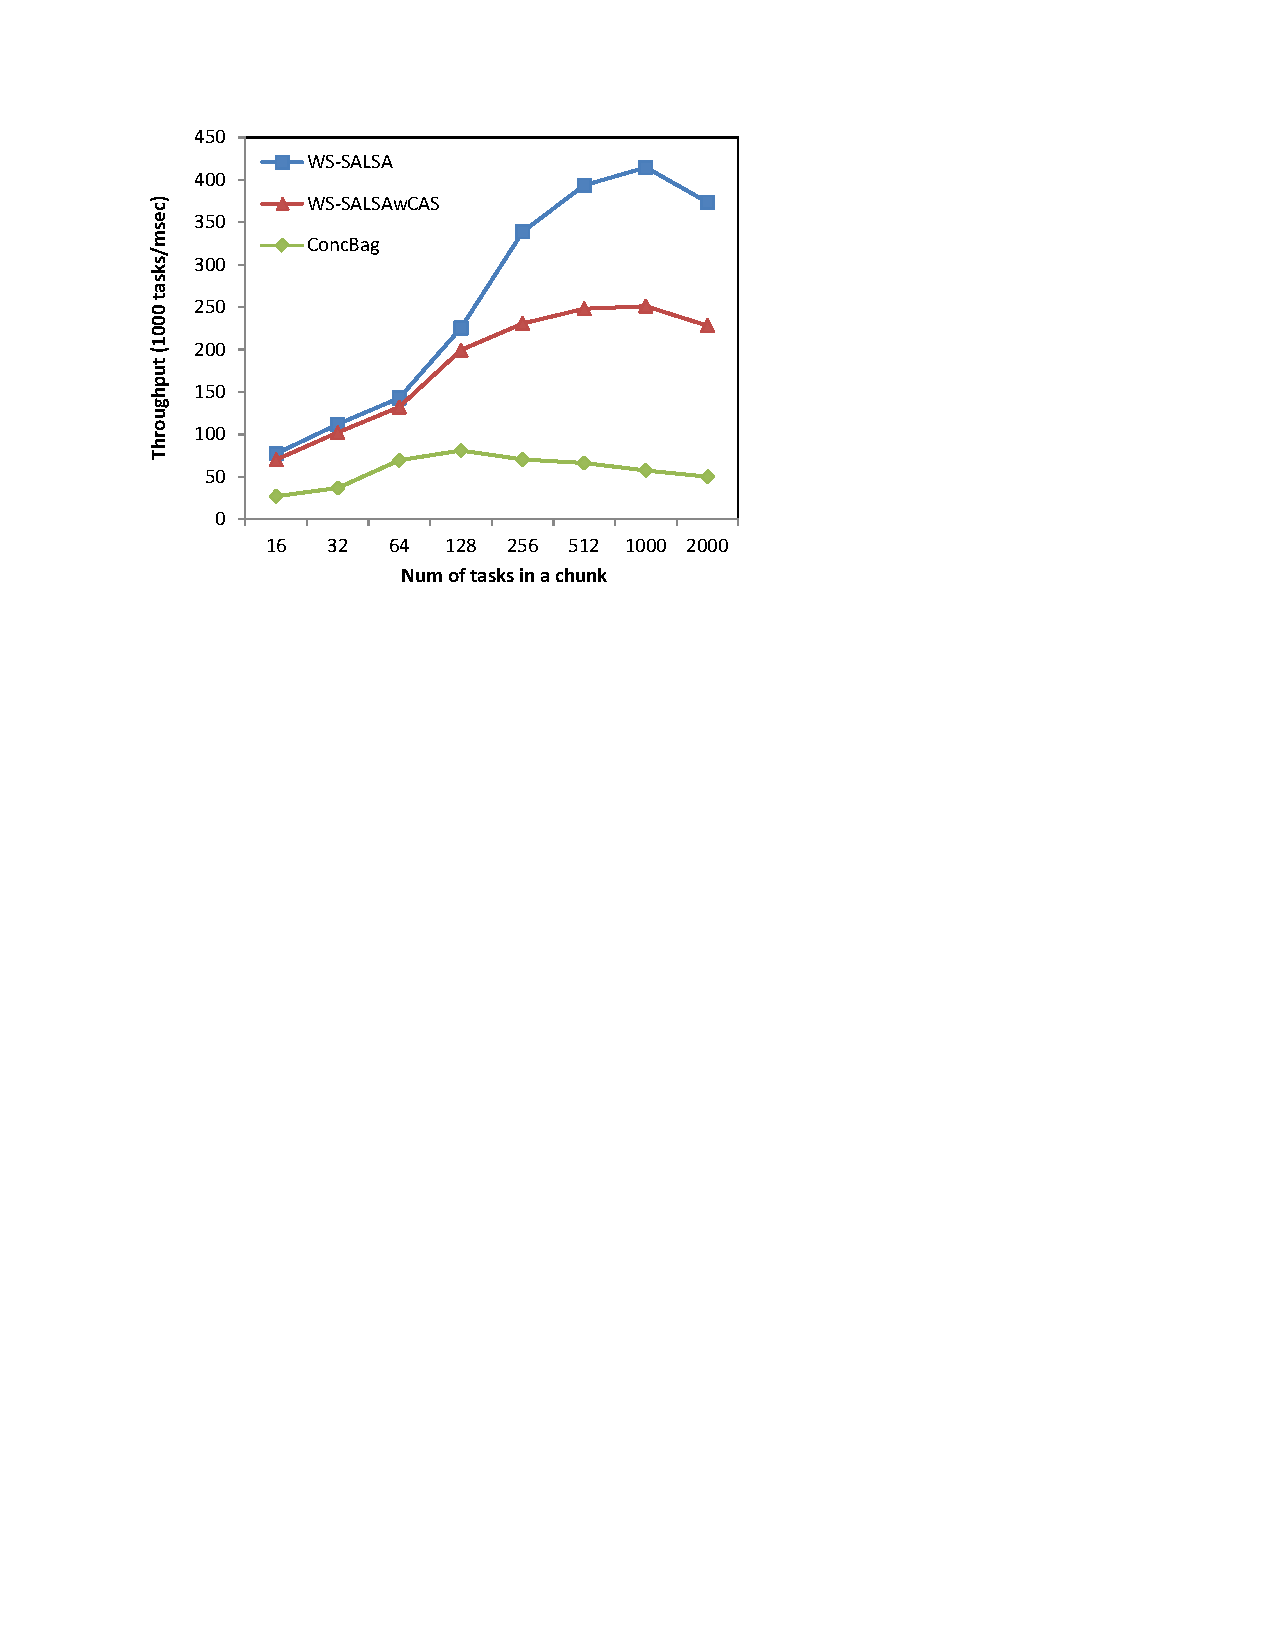
\includegraphics[width=0.45\textwidth]{figures/chunk-size}
%  \caption{\footnotesize{System throughput as a function of chunk size. }}
%	\label{fig:chunk-size}
%\end{figure}
\negspace
\section{Conclusions}
\label{sec:conclusions}
\negspace
We presented a highly-scalable task pool framework, built upon
our novel SALSA single-consumer pools and work stealing.
Our work has employed a number of novel techniques for improving
performance: 1) lightweight and synchronization-free produce and consume operations in the common case; 
2) NUMA-aware memory management, which keeps most data accesses inside NUMA nodes;
3) a chunk-based stealing approach that decreases the stealing cost and suits NUMA migration schemes; and 4) elegant producer-based
balancing for decreasing the likelihood of stealing.

We have shown that our solution scales linearly with the number
of threads. It outperforms other work-stealing techniques by a
factor of 20, and state-of-the art non-FIFO pools by a factor of 5.
We have further shown that it is highly robust to imbalances and
unexpected thread stalls.

We believe that our general approach of partitioning data structures
among threads, along with chunk-based migration and an efficient
synchronization-free fast-path, can be of benefit in building
additional scalable high-performance services in the future.
\bibliographystyle{abbrv}
\bibliography{refs}

\pagebreak \small

\begin{appendix}

\section{SALSA Lock-freedom proof}
\label{appendix:lock-freedom}
\newtheorem*{claim:lock-free}{Claim \ref{claim:lock-free}}
\begin{claim:lock-free}
If a consumer fails in $c$ steal attempts from non-empty pools, where $c$ is the number of consumers in the system, then it is guaranteed that at least one consumer in the system returns a task during that time. 
\end{claim:lock-free}

We argue that the above claim is true SALSA with the modifications describe above. Consider a consumer that invokes {\bf steal()} on a non-empty pool. This operation may fail to return a task in four cases:
\begin{enumerate}
 \item The {\bf if} statement in line~\ref{alg:line:steal-node-empty} is true. In this case all the tasks were already taken from this chunk. However, in line~\ref{alg:line:take-steal-chunk}, the steal operation took a chunk containing tasks, and therefore tasks were taken from this chunk (by other consumers) during the steal operation.
 \item The {\bf if} statement in line~\ref{alg:line:cas-steal} is true. This may occur because task$=$TAKEN or because the CAS fails. In both cases, it means that the task pointed to by $idx+1$ was taken by another consumer during the operation.
 \item The {\bf if} statement in line~\ref{alg:line:steal-chunk-not-full} is true. This means that the next available task pointed by $idx+1$ is a free slot in the chunk. However when the task was chosen in line~\ref{alg:line:take-steal-chunk}, the chunk contained a task, i.e., $idx+1$ pointed to a non-empty slot. This means that $idx$ was increased by the owner of the pool and so by the time its operation completes, it either returns the task or fails in the CAS because the task has already been returned.
 \item The {\bf if} statement in line~\ref{alg:line:chown} is true, In this case, the steal operation fails because another consumer steals this chunk. Since the consumer that stole this chunk succeed in his CAS in line~\ref{alg:line:chown}, the current case can not apply for it and therefore its operation either returns a task, or one of the above cases applies to it and therefore there is another operation that eventually returns a task. 
\end{enumerate}

In the first two cases there is another consumer that returns a task and the claim holds. In the last two cases there is another consumer which either returns a task or is running an operation which, cannot end without a task being returned. If $c-1$ steals operation do not return a task, and during that time no other consumer returns a task, we know that all the consumers are running operations that cannot finish without a task being returned, either the $c$'th steal will not be interrupted and return a task, or one of the pending operations will return a task. Therefore, when this operation ends it is guaranteed that a task will be taken from the pool and the claim holds.
\clearpage
\section{SALSA correctness}
\label{appendix:salsa-correctness}
\begin{claim}
\label{salsa-insert-claim}
 If a SALSA operation returns a task, this task has been previously inserted to a pool by a producer.
\end{claim}
\noindent
The proof of Claim~\ref{salsa-insert-claim} is immediate.

\vspace{5pt}\noindent
%Before we prove the next claim we prove the following lemmas:
\begin{lemma}
 \label{lemma:steal-take-bound}
 Let $i$ be the $idx$ of the node used by a consumer that is about to execute line~\ref{alg:lines:fast-path}. Then consumers that steal the chunk pointed by that node cannot take tasks from slots smaller than $i+1$. 
\end{lemma}
\begin{proof}
 If a consumer $c$ reached line~\ref{alg:lines:fast-path} then since the {\bf if} statement in line~\ref{alg:lines:consumer-owner-check} was true, we conclude that if a consumer stole the chunk it saw the value $i$ that $c$ uses in line~\ref{alg:lines:fast-path} because the stealer reads this value \emph{after} changing ownership. Since the stealer only take tasks from slots greater than the value it read, we deduce that it only take tasks from slots greater than $i$.
\end{proof}

\begin{lemma}
 \label{lemma:no-inc-after-steal}
 Let $i$ be the $idx$ of a node as read by a stealing consumer after changing chunk ownership in line~\ref{alg:line:chown}. Then the previous owner of the chunk cannot take tasks in slots with index greater than $i+1$ as long as the ownership does not change.
\end{lemma}
\begin{proof}
Once a consumer notices that its chunk was stolen it sets $currentNode$ to $\bot$ (line~\ref{alg:line:check-owner-stealer}) or leaves it as $\bot$ (line~\ref{alg:lines:stolen-chunk-end}). If a consumer takes a Node from its pool, it makes sure that it is the owner of this Node's chunk, i.e., when a consumer notices that a chunk has been stolen it stops using the node that pointed to it.

If a consumer increases the $idx$ of a Node, it checks if it is still its owner (lines~\ref{alg:lines:consumer-owner-check} and~\ref{alg:line:check-owner-stealer}). Therefore, once the ownership of a chunk changes, the $idx$ of a Node that pointed to that chunk before it was stolen, can increase by at most 1. Hence, the value of $i$ is at least $idx-1$.

When a consumer takes a task in {\bf consume()} (lines~\ref{alg:lines:fast-path} and~\ref{alg:line:cas-consumer}), it takes it from slot $k$, where $k$ is the current $idx$ of the current consumer's Node. Since we know that after a {\bf steal()} operation the $idx$ value $i$ that is read by the stealer is at least $k-1$, we conclude that the previous owner of the chunk can take tasks only from slots less than $i+1$, unless it steals this chunk again.

When a consumer takes a task in {\bf steal()}, it takes it from slot $k+1$ and then increments $idx$. Therefore, when another consumer steals this chunk, the value $i$ that it reads~\ref{alg:line:copy-prev-node} is at least $k$. As shown earlier, the original owner will not take a task greater than $k+1$ without stealing this chunk again. 
\end{proof}

\begin{claim}
\label{salsa-consumer-claim}
A task in a SALSA pool may be only returned once.
\end{claim}

\begin{proof}
A consumer returns a task only after it changes the value of the task slot to TAKEN. 
Therefore, it is sufficient to show that only one consumer can change a given slot to TAKEN.
There are three places in the code a value can be changed to TAKEN (see Algorithm~\ref{alg:non-fifo}):
\begin{enumerate}
 \item Line~\ref{alg:line:cas-consumer} -- a consumer detected that the chunk has been stolen and therefore performs a CAS operation to mark the slot as TAKEN.
 \item Line~\ref{alg:line:cas-steal} -- a consumer attempts to take a task using CAS operation after it steals a chunk.
 \item Line~\ref{alg:lines:fast-path} -- a consumer tries to take a task without synchronization (fast-path).
\end{enumerate}

When multiple consumers try to take a task using CAS operations, only one can succeed, therefore, it is enough to show that the operation that does not use CAS, cannot compete with other operations that try to take the same task.

We now show that if the operation in line~\ref{alg:lines:fast-path} takes a task, no other operation takes this task. 
Consider a consumer $a$ that is about to execute line~\ref{alg:lines:fast-path}.
According to Lemma~\ref{lemma:steal-take-bound}, consumers that steal the chunk used by $a$, cannot take the task that $a$ is about to take.

After stealing a Node, the consumer increases $idx$ by 1 (see line~\ref{alg:line:steal-idx-inc}), and therefore the next time it invokes {\bf consume()} it will take the task from $i+2$ where $i$ is the value it read from the previous Node in line~\ref{alg:line:copy-prev-node}. Therefore, in case $a$ stole from another consumer $b$, when $a$ executes line~\ref{alg:line:copy-prev-node}, then $b$ can only take tasks from slots smaller than $i+2$. Hence, $b$ cannot take the task that $a$ retrieves in line~\ref{alg:lines:fast-path} unless it resteals the chunk. 
\end{proof}

\clearpage
\section{Chunk size influence}
\label{appendix:chunk-size}
\begin{figure}[htb]
 \begin{center}
   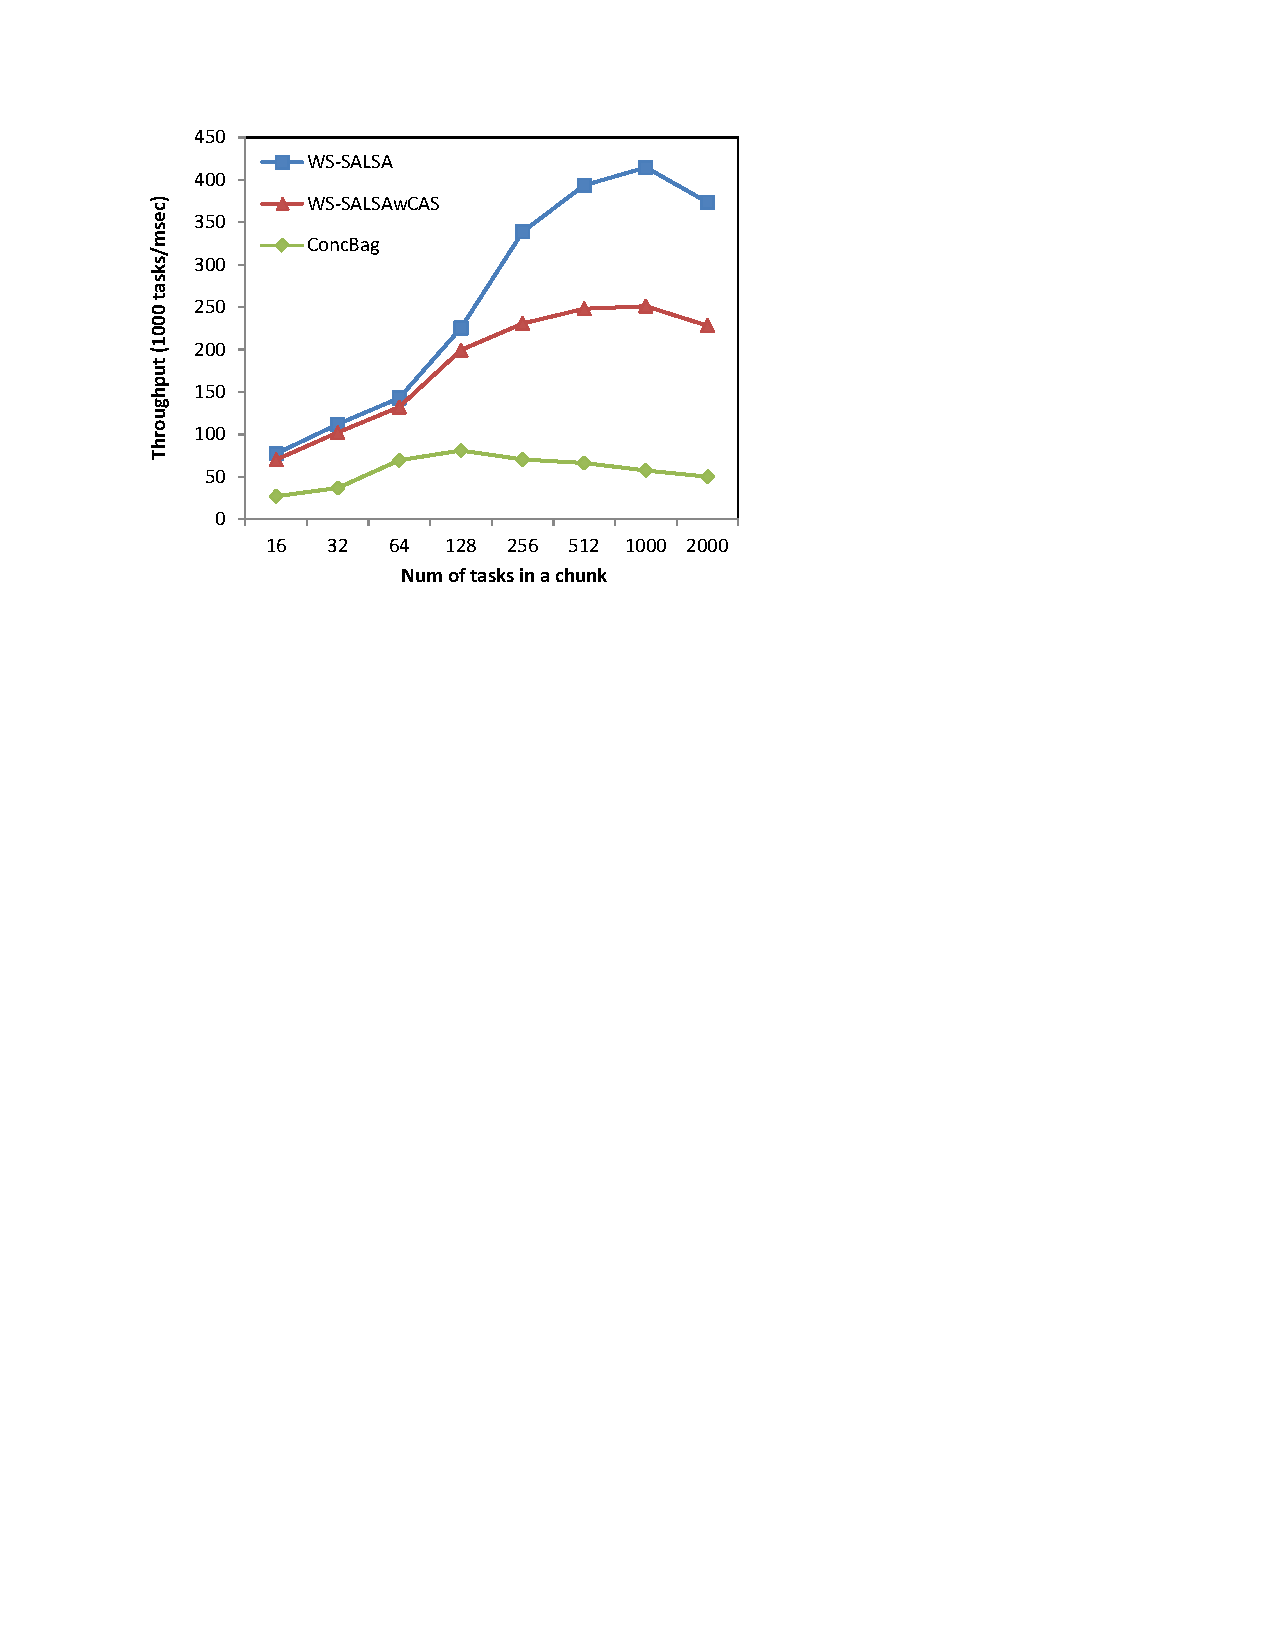
\includegraphics[width=0.45\textwidth]{figures/chunk-size}
 \end{center}
	\caption{\footnotesize{System throughput as a function of the chunk size. }}
	\label{fig:chunk-size}
\end{figure}
Figure~\ref{fig:chunk-size} shows the influence of the chunk size on system throughput for the chunk-based algorithms SALSA, SALSA+CAS and ConcBags in the $16/16$ workload. 
SALSA variations achieve their best throughput for large chunks with $1000$ tasks ($\sim8$KB size in $64$-bit architectures). The optimal chunk for ConcBags includes $128$ tasks. We believe that the reason that ConcBags cannot handle large chunk sizes is related to the fact that a consumer should linearly scan a chunk when seeking for a task to steal. In contrast, SALSA's algorithm of fast-path consumption keeps the index of the latest consumed task in the chunk node and therefore its consume operations terminate in $O(1)$ steps for every chunk size. 
In our evaluation we used optimal chunk sizes for each algorithm. 


\end{appendix}

\end{document}